%%%%%%%%%%%%%%%%%%%%%%%%%%%%%%%%%%%%%%%%%%%%%%%%%%%%%%%%%%%%%%%%%%%%%%
%%
%% This LaTeX file typesets the User's Guide for fbe_tez.sty.
%%
%%%%%%%%%%%%%%%%%%%%%%%%%%%%%%%%%%%%%%%%%%%%%%%%%%%%%%%%%%%%%%%%%%%%%%
%%
%% COPYRIGHT 1999, 2001, 2003 by
%% Feza Kerestecioglu <kerestec@boun.edu.tr>
%%
%% Copying of part or all of any file in the fbe_tez package is
%% allowed under the following conditions only:
%% (1) You may freely distribute unchanged copies of the files. Please
%%     include the documentation when you do so.
%% (2) You may modify a renamed copy of any file, but only for your
%%     personal use.
%% (3) You may copy fragments from the files, for personal use only
%%     and as long as credit is given where credit is due.
%%
%% You are NOT ALLOWED to take money for the distribution or use of
%% these files or modified versions or fragments thereof.
%%
%%%%%%%%%%%%%%%%%%%%%%%%%%%%%%%%%%%%%%%%%%%%%%%%%%%%%%%%%%%%%%%%%%%%%%
%

\documentclass[12pt]{article}
\usepackage{amsmath}
\usepackage{algorithm}
\usepackage[noend]{algpseudocode}
\usepackage{float}
\usepackage[bottom]{footmisc}
\usepackage{cite}
\usepackage{graphicx}
\usepackage{longtable}
\usepackage[utf8]{inputenc}
\usepackage[T1]{fontenc}
\graphicspath{{figures/}} % Graphics will be here

\usepackage{hyperref}
\hypersetup{
    colorlinks=true,
    linkcolor=blue,
    filecolor=magenta,      
    urlcolor=cyan,
}

%
% Pagestyle
%
\oddsidemargin9.6mm
\evensidemargin9.6mm
\topmargin-1cm
\headheight20pt
\textwidth155mm
\textheight232mm
\pagestyle{myheadings}
%
% Macros
%
\newcommand\fbe{{\tt fbe\_tez}}
\newcommand\report{{\tt report}}
\newcommand{\bq}{\begin{quotation}\noindent}
\newcommand{\eq}{\end{quotation}}
\renewcommand{\arg}[1]{$\langle\mbox{\it #1}\rangle$}
%
% Title declarations
%

\title{{\Huge CmpE 443 Final Project Design Document} \\ Group Name : Doğan SLX  }
\author{Members \\ Emirhan SARAÇ (Team Leader) \\ Muhammed Fatih BALIN\\ Yusuf BAŞPINAR \\ Enis SİMSAR }
\date{December 28, 2018 \\ Version 1.00}
%
\begin{document}
\maketitle
\break
\tableofcontents
\newpage
\section{Introduction}
Our GitHub Resository: \newline \url{https://github.com/443-Embedded/embedded-final-project} \newline
Doğan SLX component is an embedded system for a car with joystick controller for manual mode or autonomous mode. 
Joystick, UART and WIFI is an input type component. It takes the input from user and transfer it to the board. We used two motor speed sensor for each side: right and left. We have LEDs, LDRs and Motor Driver Controller components for output. Actions:

\subsection{Manual Mode}
\begin{itemize}
    \item The robot will be at stop phase (output), when robot enters the manual mode (input, push button or UART or WIFI).
    \item When Joystick Left button is pressed (input), starts in counter-clockwise direction (output) and blink left LEDs (output).
    \item When Joystick Up button is pressed (input), starts to travel in forward direction (output) and turn on front LEDs (output).
    \item When Joystick Down button is pressed (input), starts to travel in backward direction (output) and turn on back LEDs (output).
    \item When Joystick Center button is pressed (input), stops (output).
    \item When Joystick Right button is pressed (input), starts in clockwise direction (output) and blink right LEDs (output).
    \item While going in forward direction, if ultrasonic sensor detects an obstacle (its direction is parametric in parameters.h file) (output for trigger pin and echo for echo pin), robot moves backward (output) until a length which is parametric and stop (output).
    \item Trimpot resistor can change the speed of the robot. (getting information input, adjusting the speed according to its value output)/
    \item If the robot detect a light source while going in forward direction (input from LDRs), it escape from the light source (adjusting leds and motor speeds and directions.) (output)
\end{itemize}

\subsection{Auto Mode}
\begin{itemize}
    \item The robot will be at stop phase (output), when robot enters the auto mode (input, push button or UART or WIFI).
    \item The robot will be start with two different ways: pressing joystick up button (input) or sending 66 via UART or WIFI (input). Then, robot will be start. (output) (forward leds and forward direction movement). The robot go along the road. 
    \item While going in forward direction, if ultrasonic sensor detects an obstacle (its direction is parametric in parameters.h file) (output for trigger pin and echo for echo pin), robot moves backward (output) until a length which is parametric and stop (output).
    \item Trimpot resistor can change the speed of the robot. (getting information input, adjusting the speed according to its value output)/
    \item If the robot detect a light source while going in forward direction (input from LDRs), it escape from the light source (adjusting leds and motor speeds and directions.) (output)
\end{itemize}

\break

\section{Block Diagram}
\begin{figure}[htbp]
\begin{center}
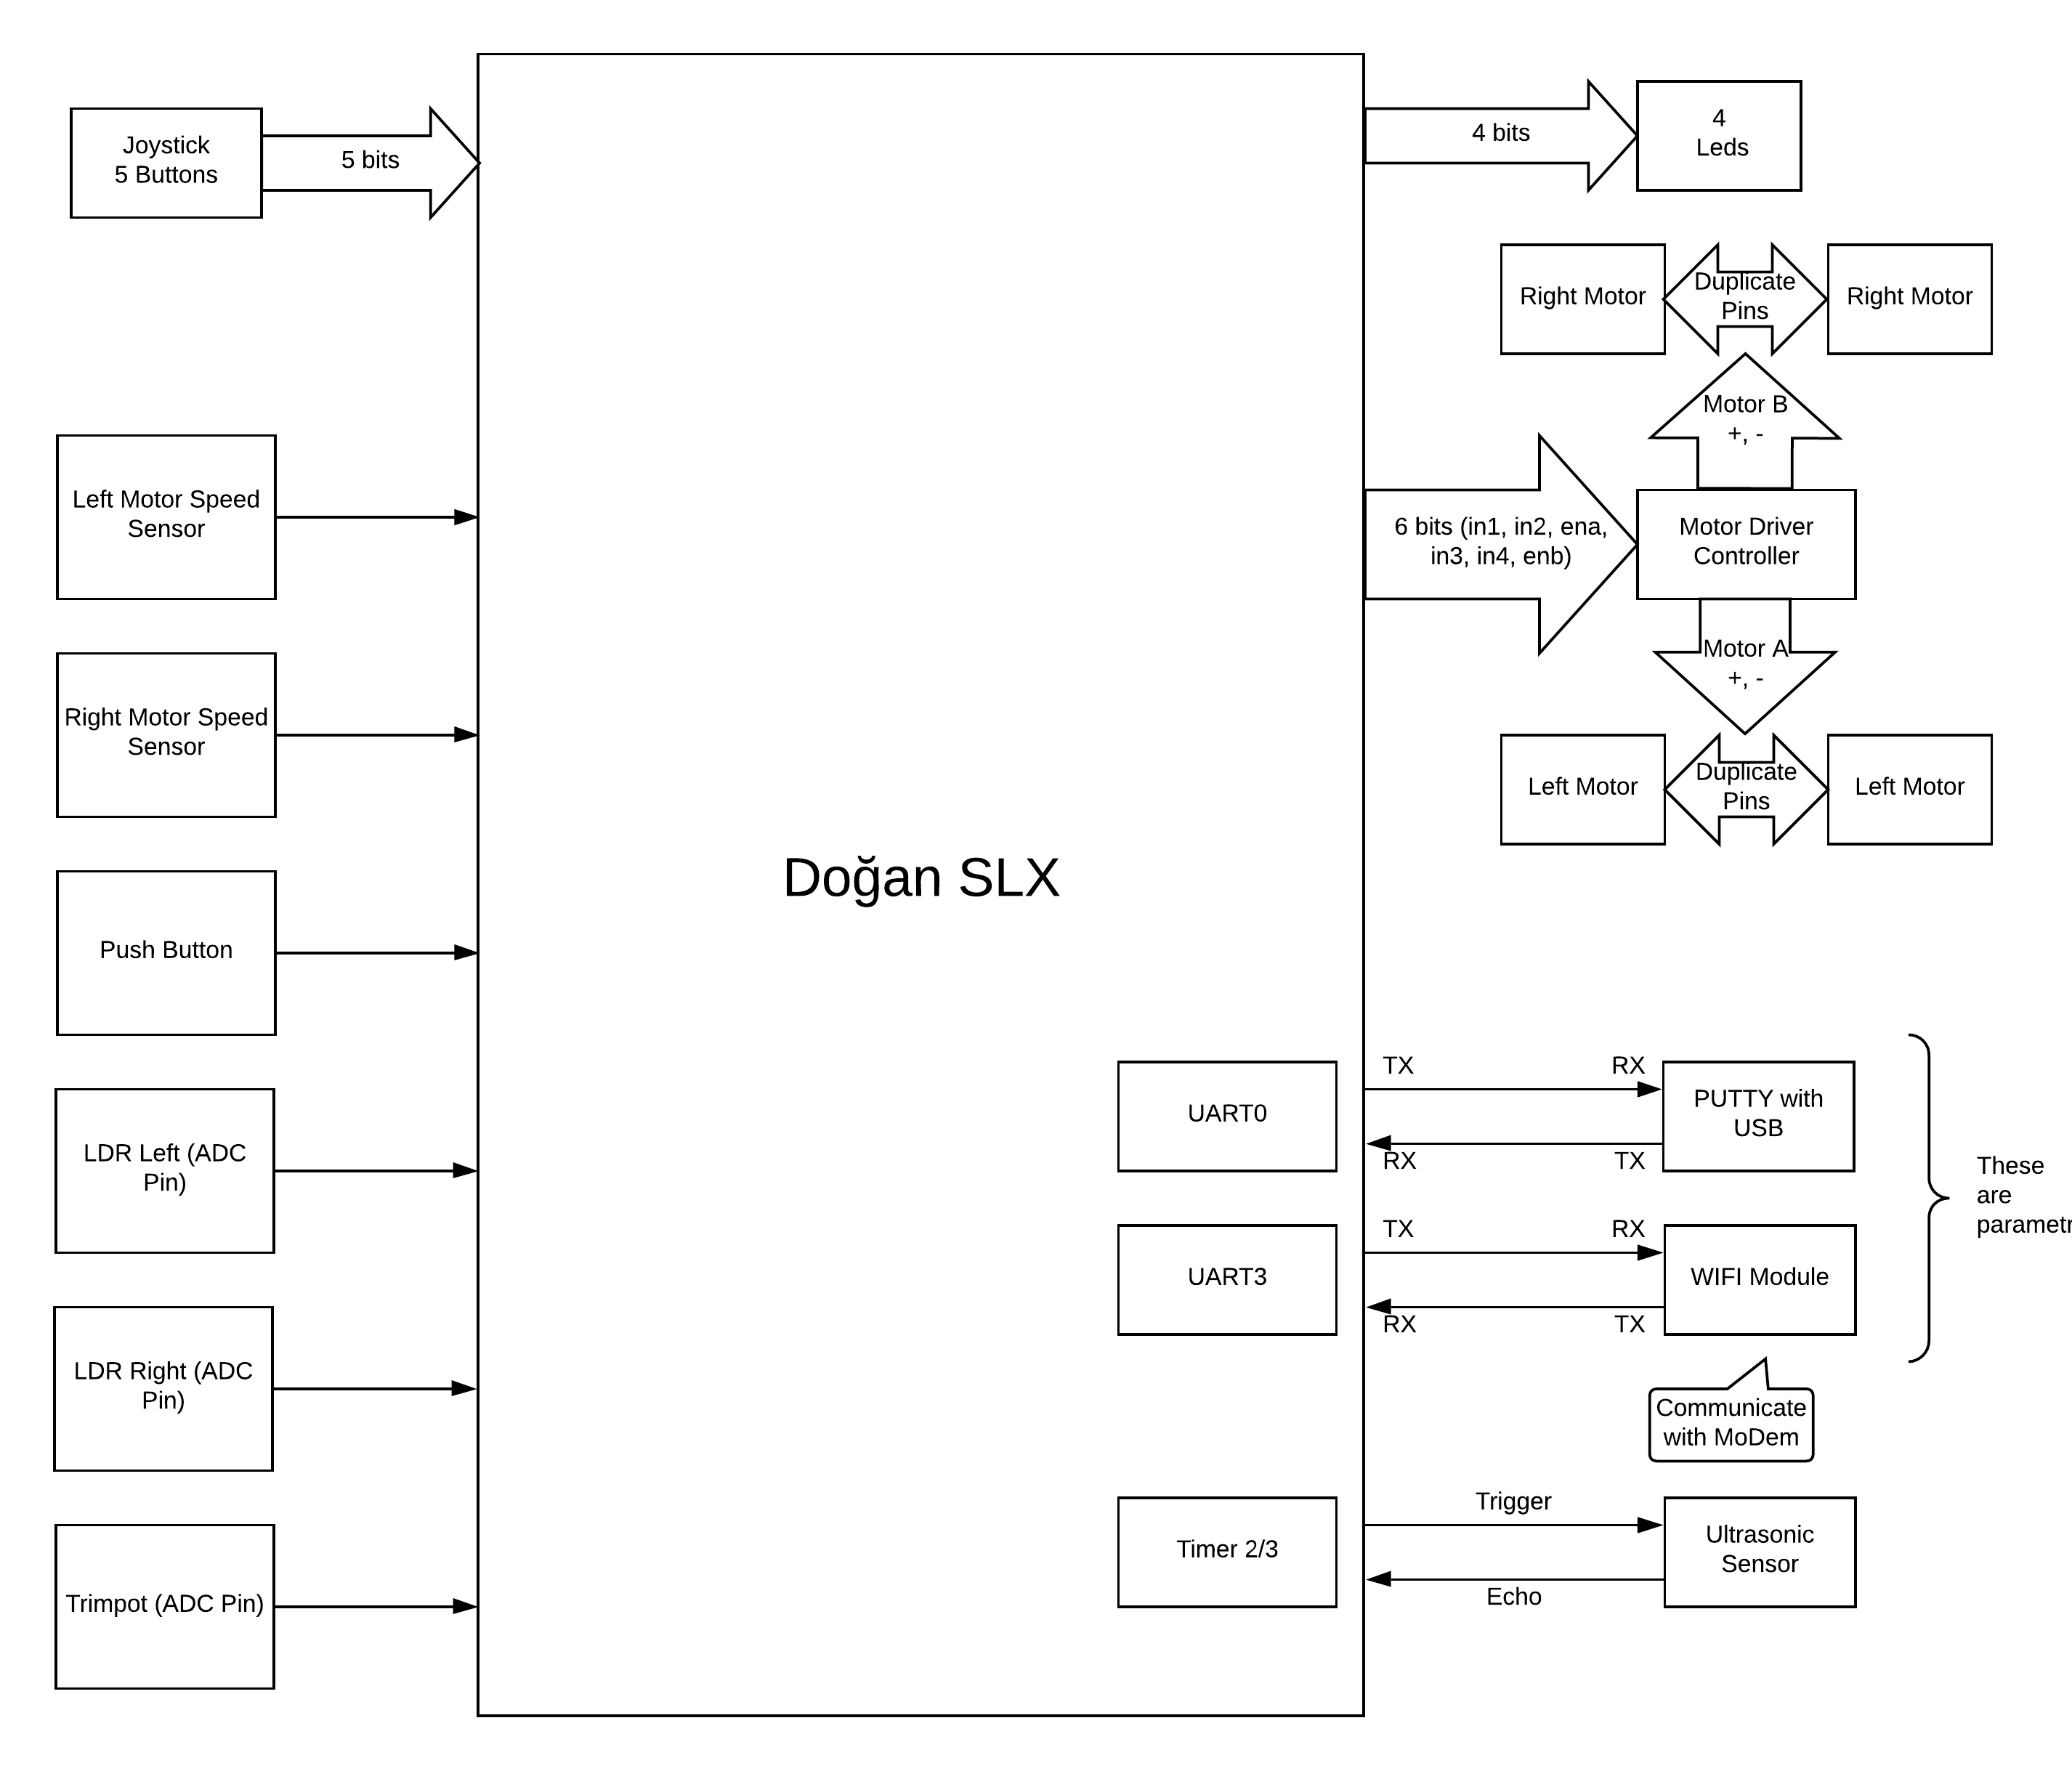
\includegraphics[width=1\columnwidth]{block_diagram.png}
\end{center}
\caption{Block Diagram}
\vskip\baselineskip % Leave a vertical skip below the figure
\label{fig:sample1}
\end{figure}

\break

\section{System-Level Functional Diagram}
For big version click \href{https://drive.google.com/open?id=1dWiSfpzXYaefMXwWXXsjY_Xs9vBozmQ6}{here.}

\begin{figure}[htbp]
\begin{center}
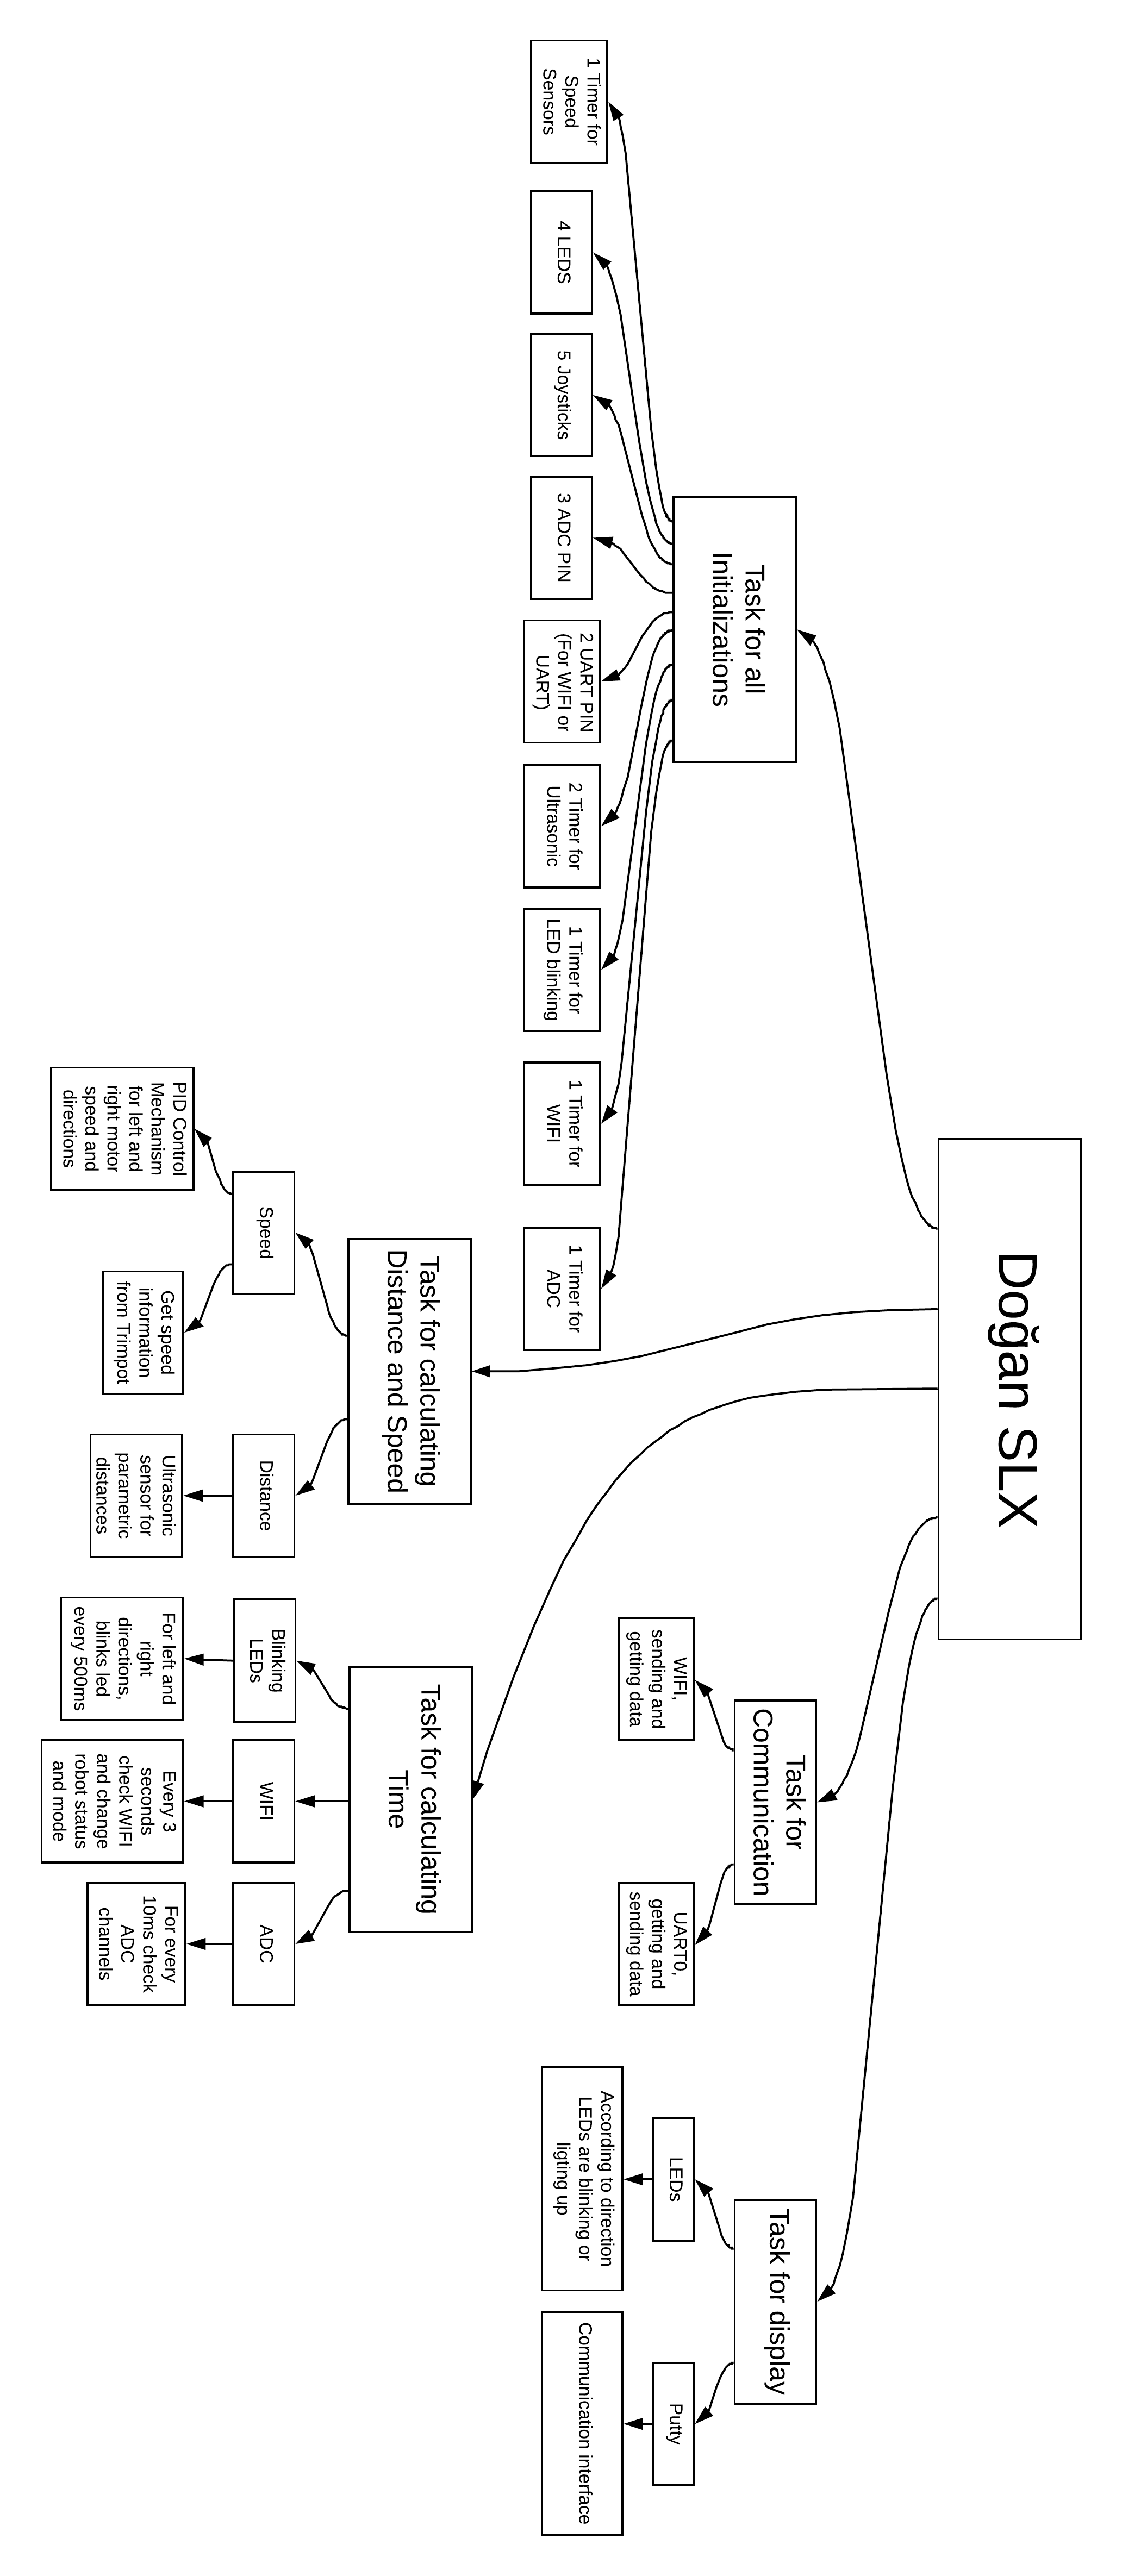
\includegraphics[height=1\columnwidth]{system_level_diagram.png}
\end{center}
\caption{System-Level Functional Diagram}
\vskip\baselineskip % Leave a vertical skip below the figure
\label{fig:sample2}
\end{figure}

\newpage
\section{Sequence Diagram}
\subsection{Manual Mode Diagrams}
\begin{figure}[htbp]
\begin{center}
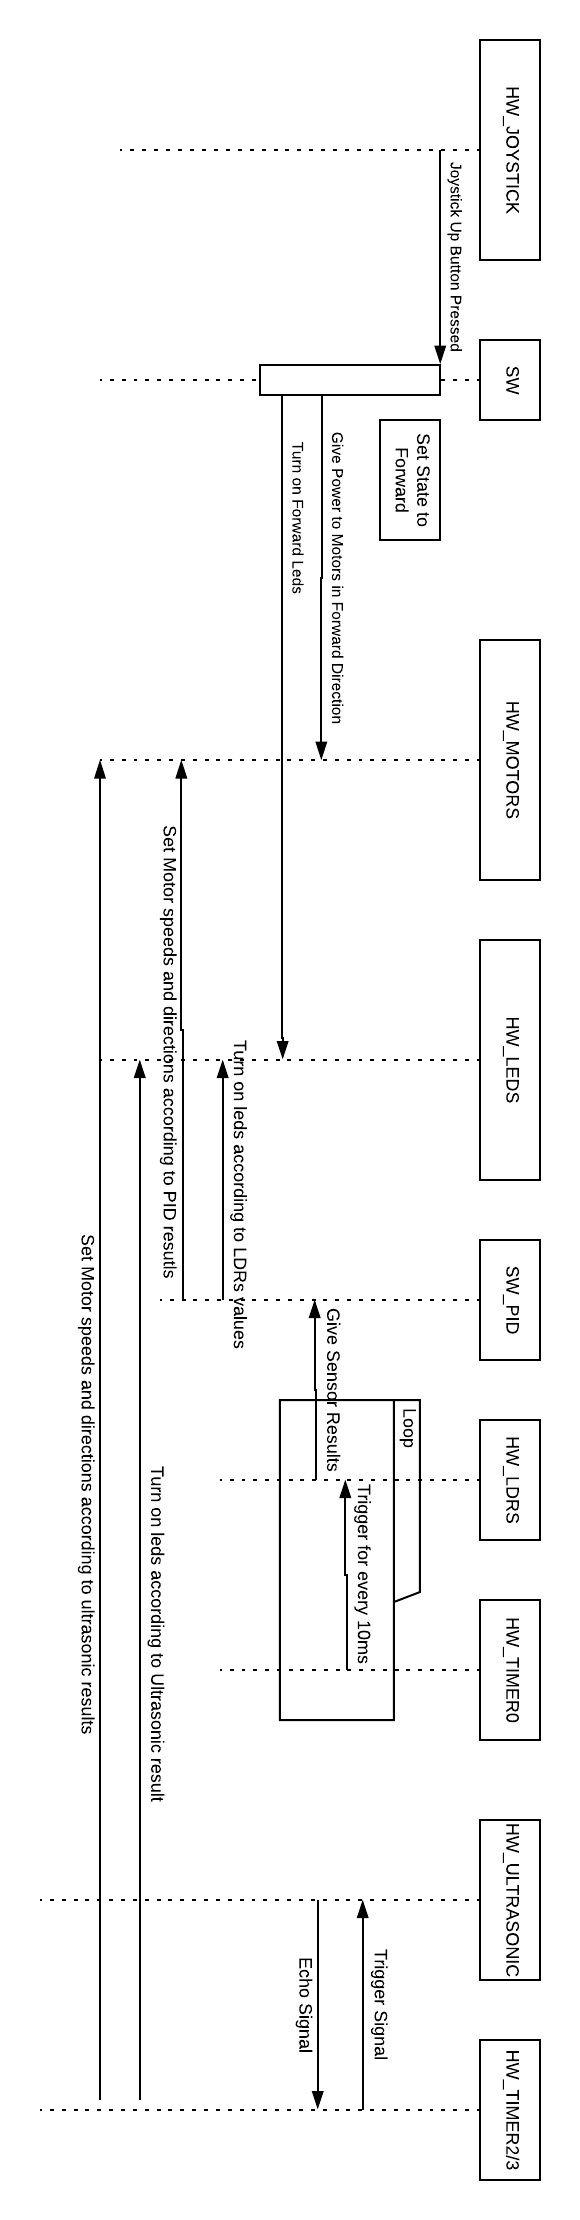
\includegraphics[height=1\columnwidth]{sequence_diagram_forward.png}
\end{center}
\caption{Forward Sequence Diagram}
\vskip\baselineskip % Leave a vertical skip below the figure
\label{fig:forward_sequence}
\end{figure}

\begin{figure}[htbp]
\begin{center}
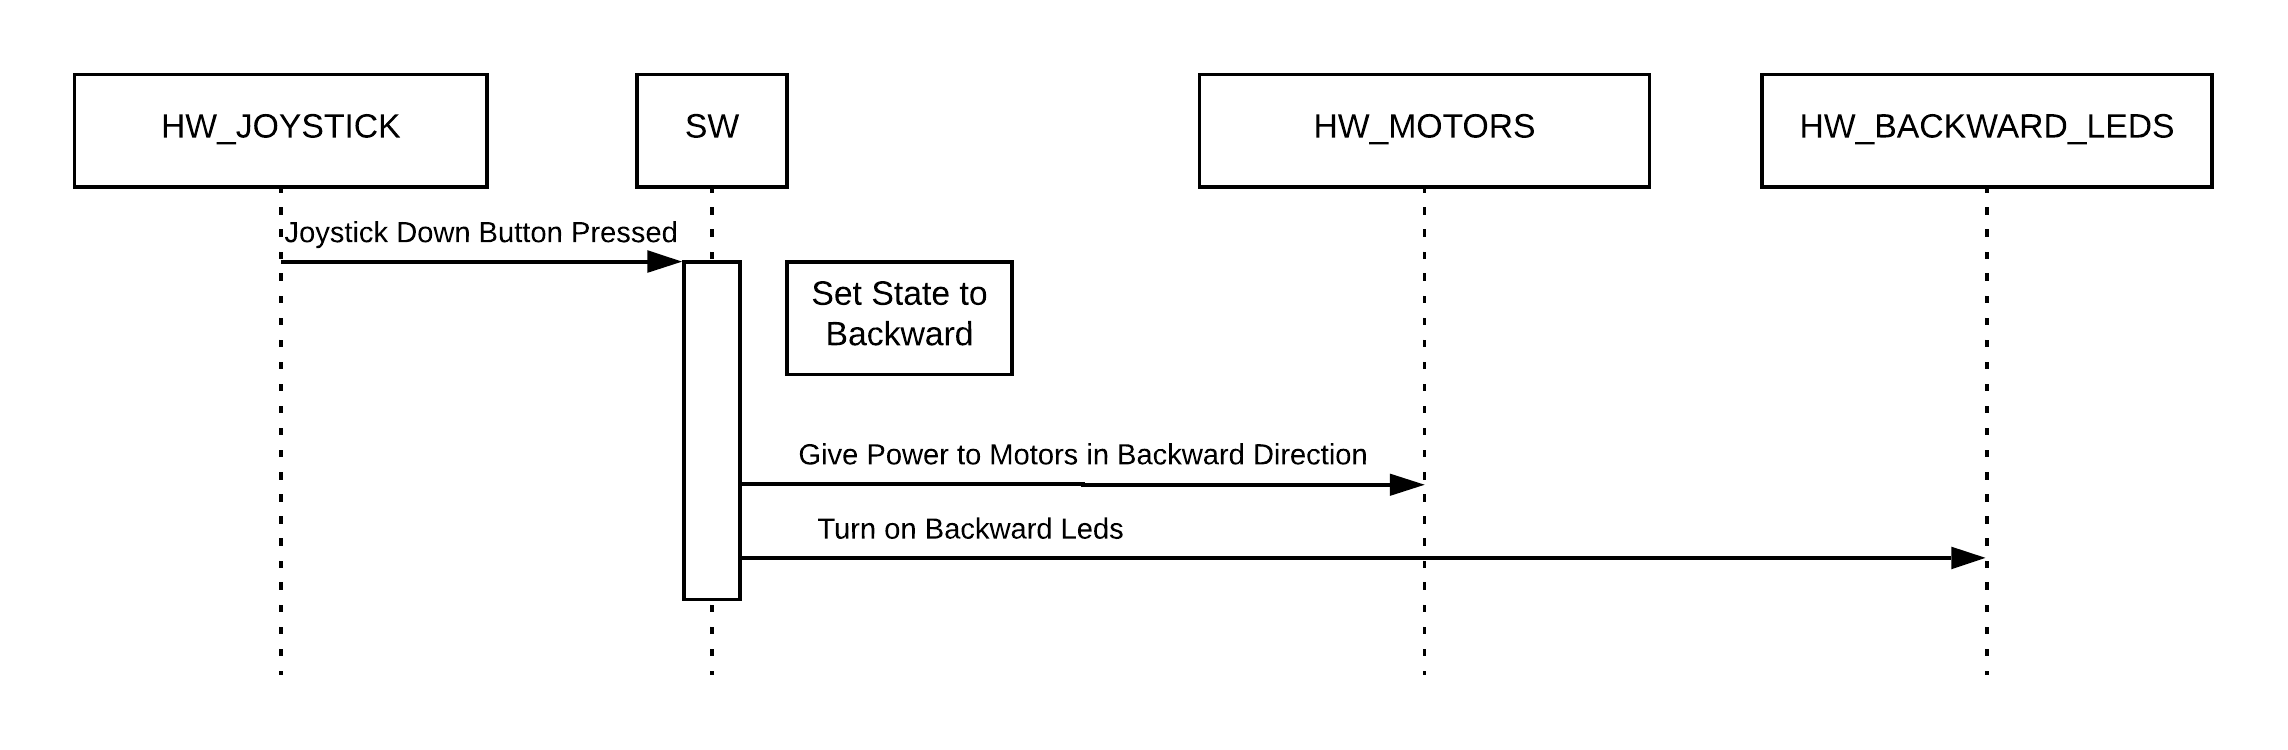
\includegraphics[width=1\columnwidth]{sequence_diagram_backward.png}
\end{center}
\caption{Backward Sequence Diagram}
\vskip\baselineskip % Leave a vertical skip below the figure
\label{fig:backward_sequence}
\end{figure}

\begin{figure}[htbp]
\begin{center}
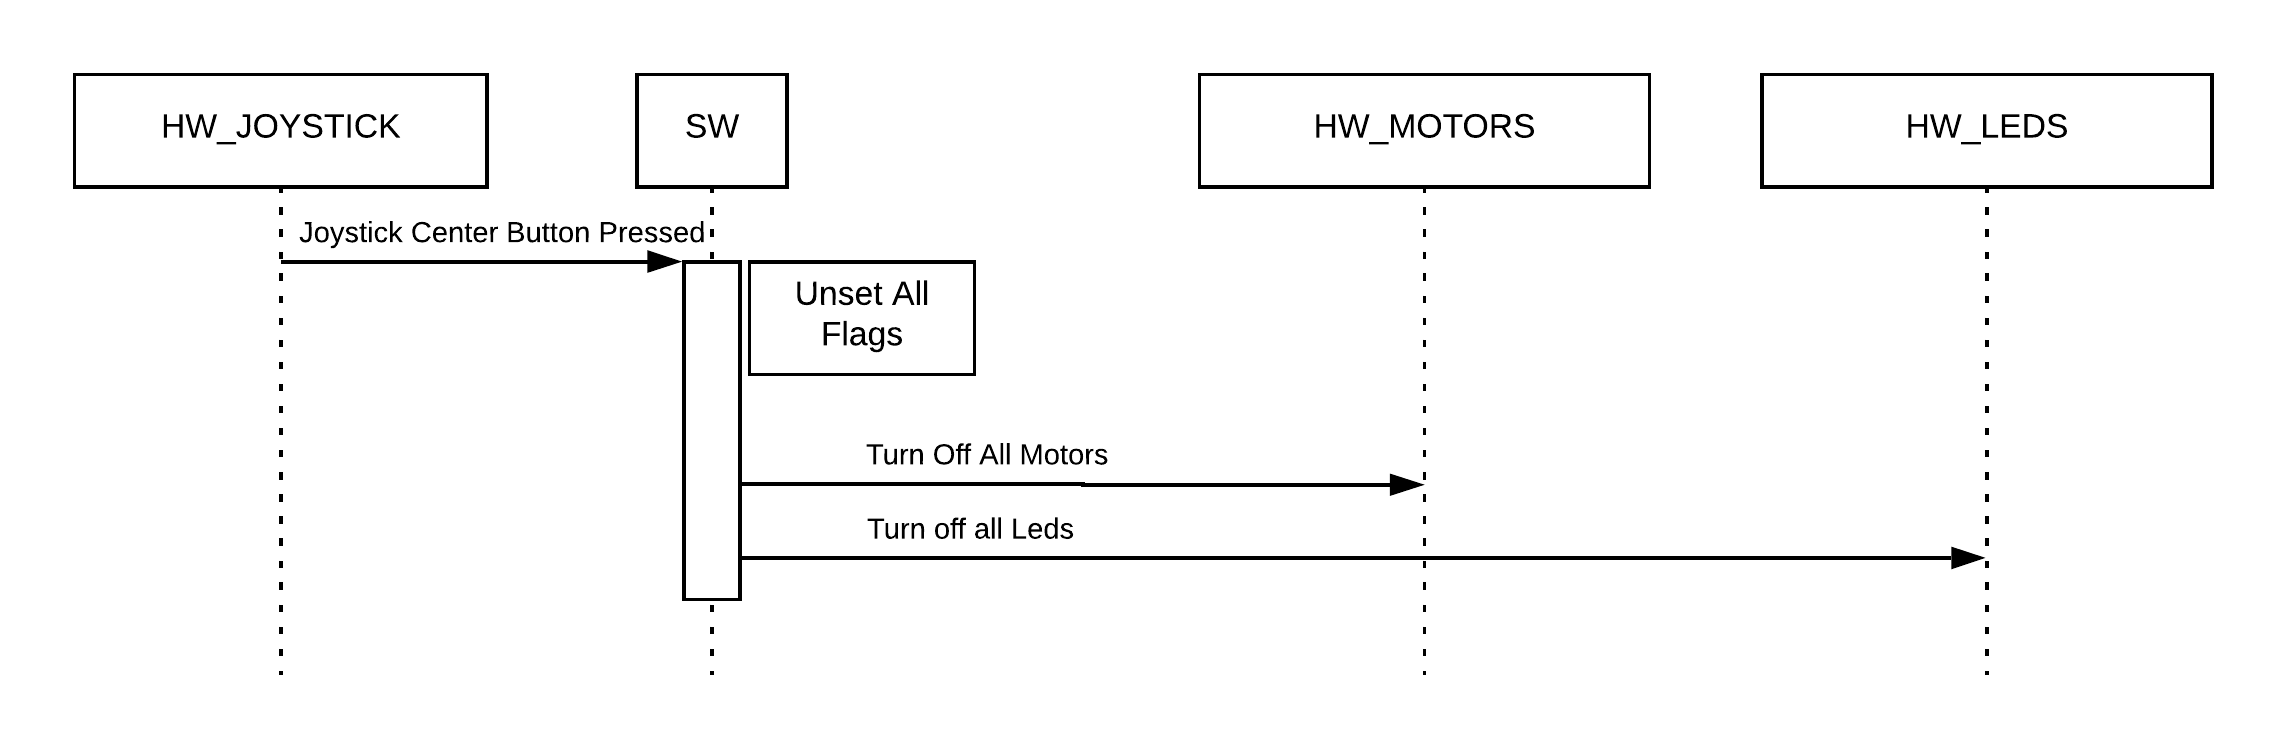
\includegraphics[width=1\columnwidth]{sequence_diagram_stop.png}
\end{center}
\caption{Stop Sequence Diagram}
\vskip\baselineskip % Leave a vertical skip below the figure
\label{fig:stop_sequence}
\end{figure}

\begin{figure}[htbp]
\begin{center}
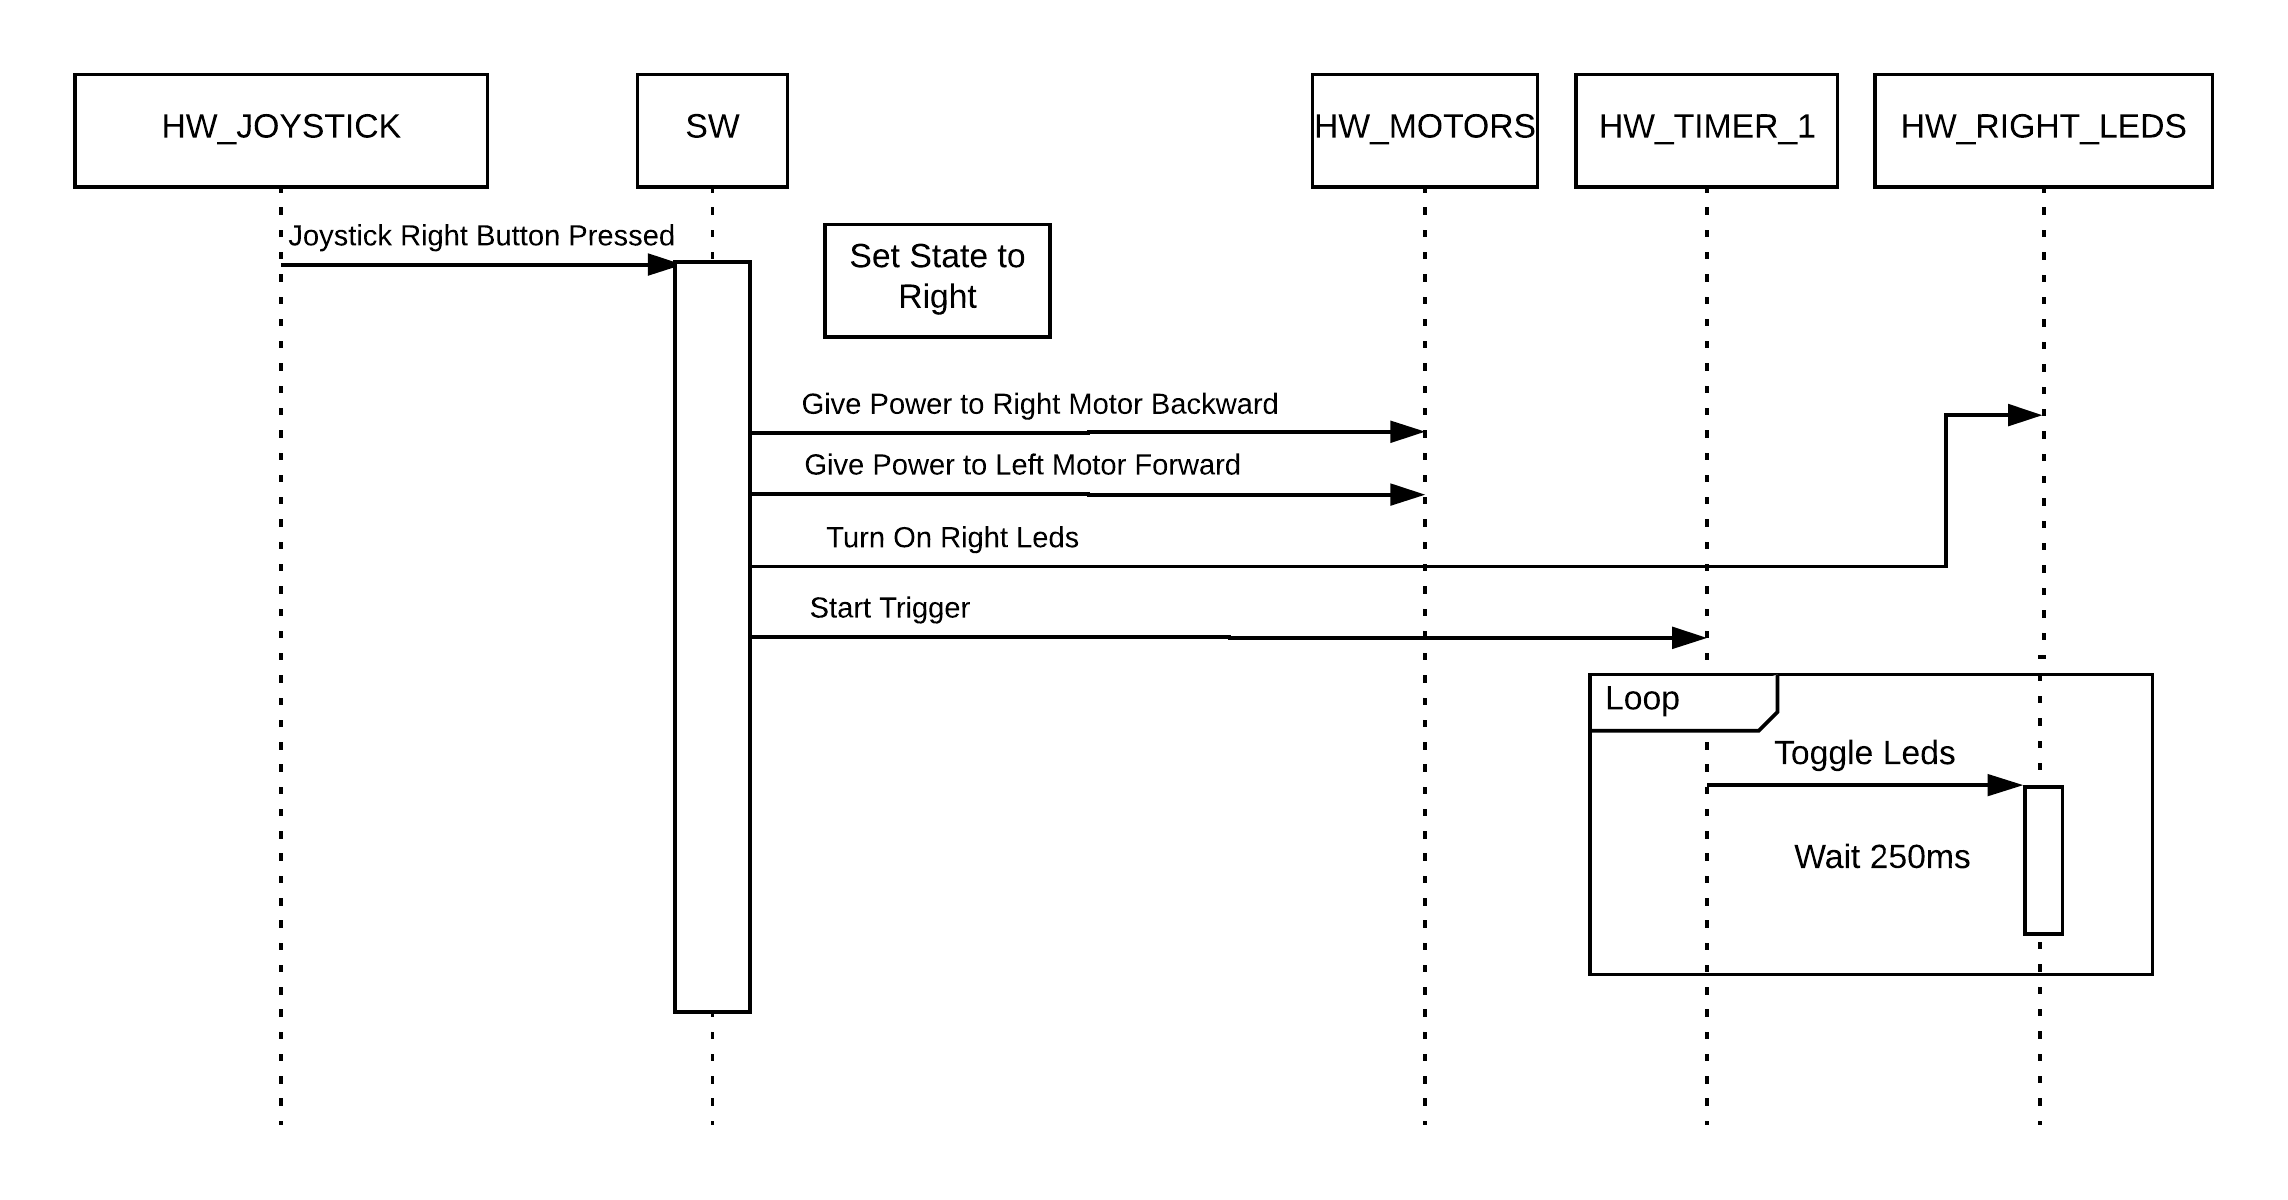
\includegraphics[width=1\columnwidth]{sequence_diagram_right.png}
\end{center}
\caption{Right Sequence Diagram}
\vskip\baselineskip % Leave a vertical skip below the figure
\label{fig:right_sequence}
\end{figure}

\begin{figure}[htbp]
\begin{center}
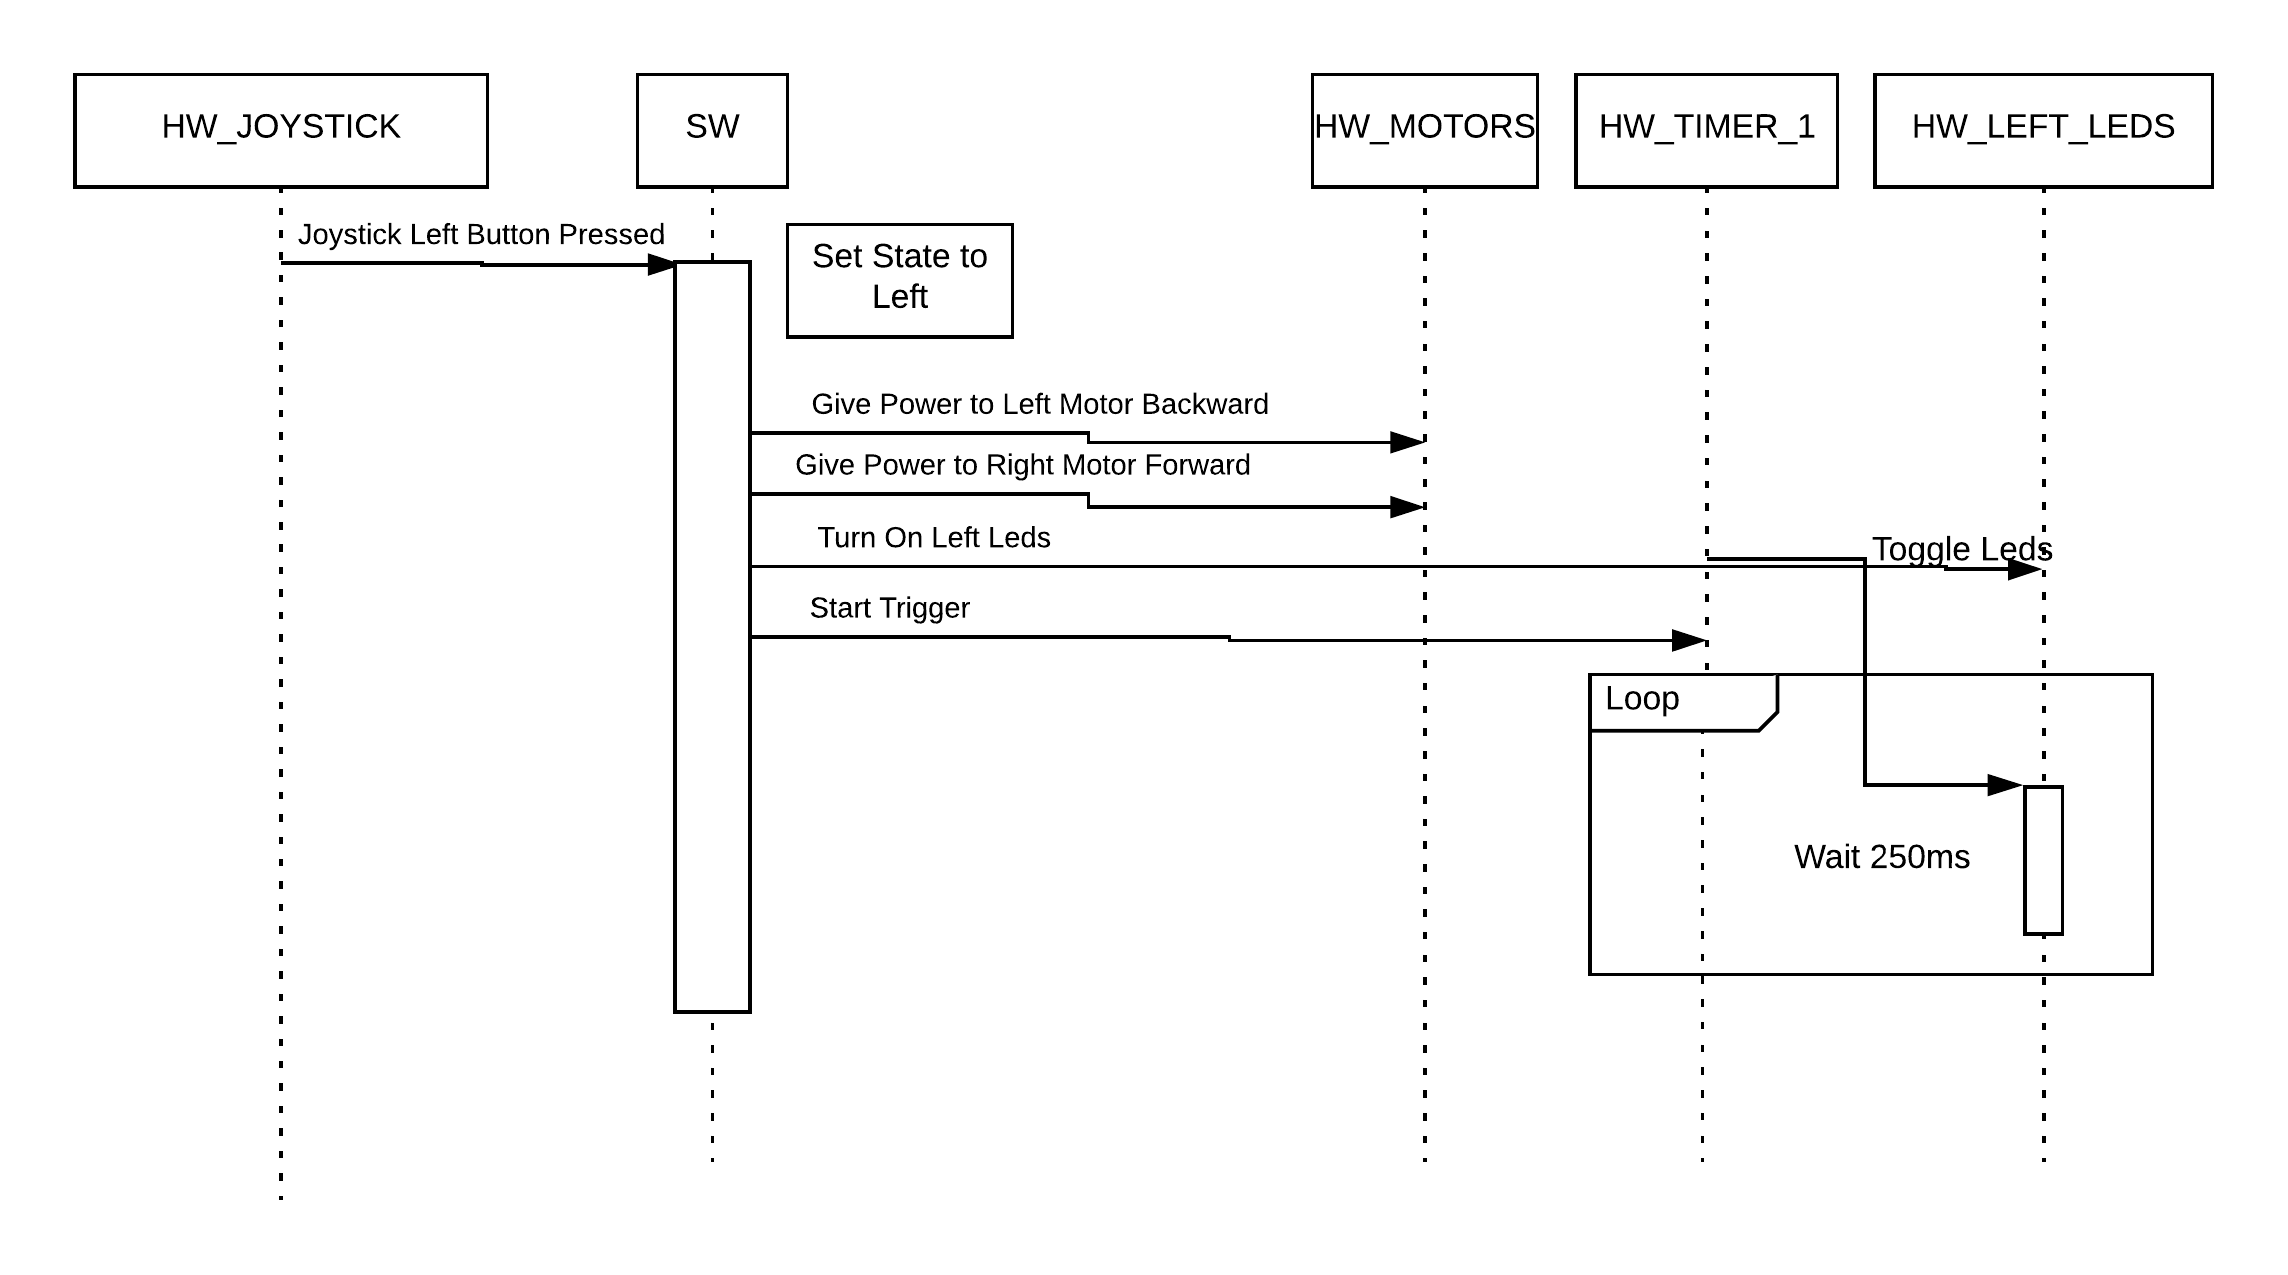
\includegraphics[width=1\columnwidth]{sequence_diagram_left.png}
\end{center}
\caption{Left Sequence Diagram}
\vskip\baselineskip % Leave a vertical skip below the figure
\label{fig:left_sequence}
\end{figure}

\break
\newpage

\subsection{Auto Mode Diagrams}
\begin{figure}[htbp]
\begin{center}
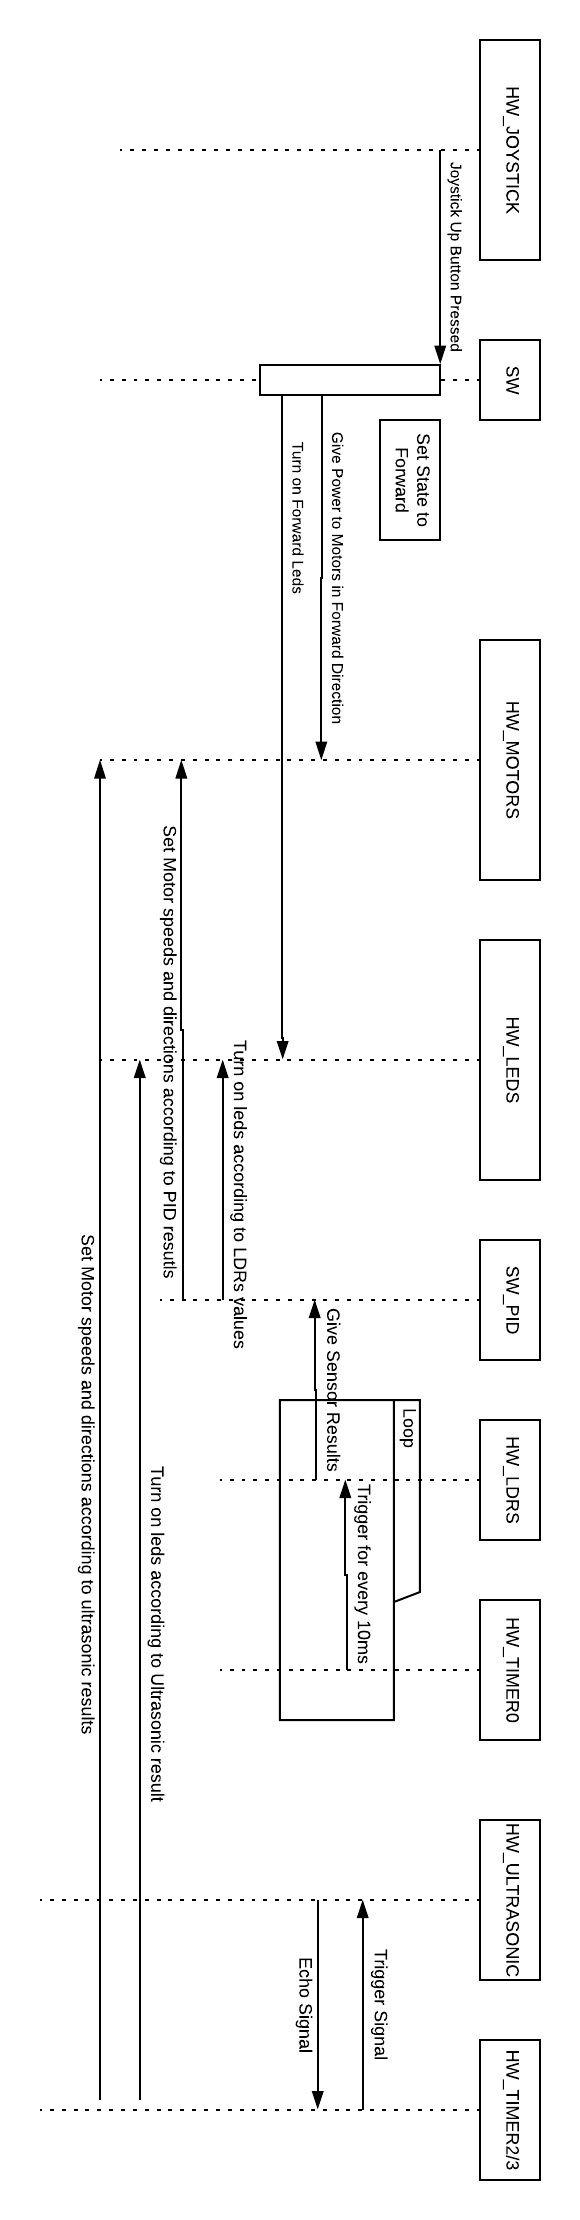
\includegraphics[height=1\columnwidth]{sequence_diagram_forward.png}
\end{center}
\caption{Forward Sequence Diagram for AUTO Mode}
\vskip\baselineskip % Leave a vertical skip below the figure
\label{fig:forward_sequence_auto}
\end{figure}

\begin{figure}[htbp]
\begin{center}
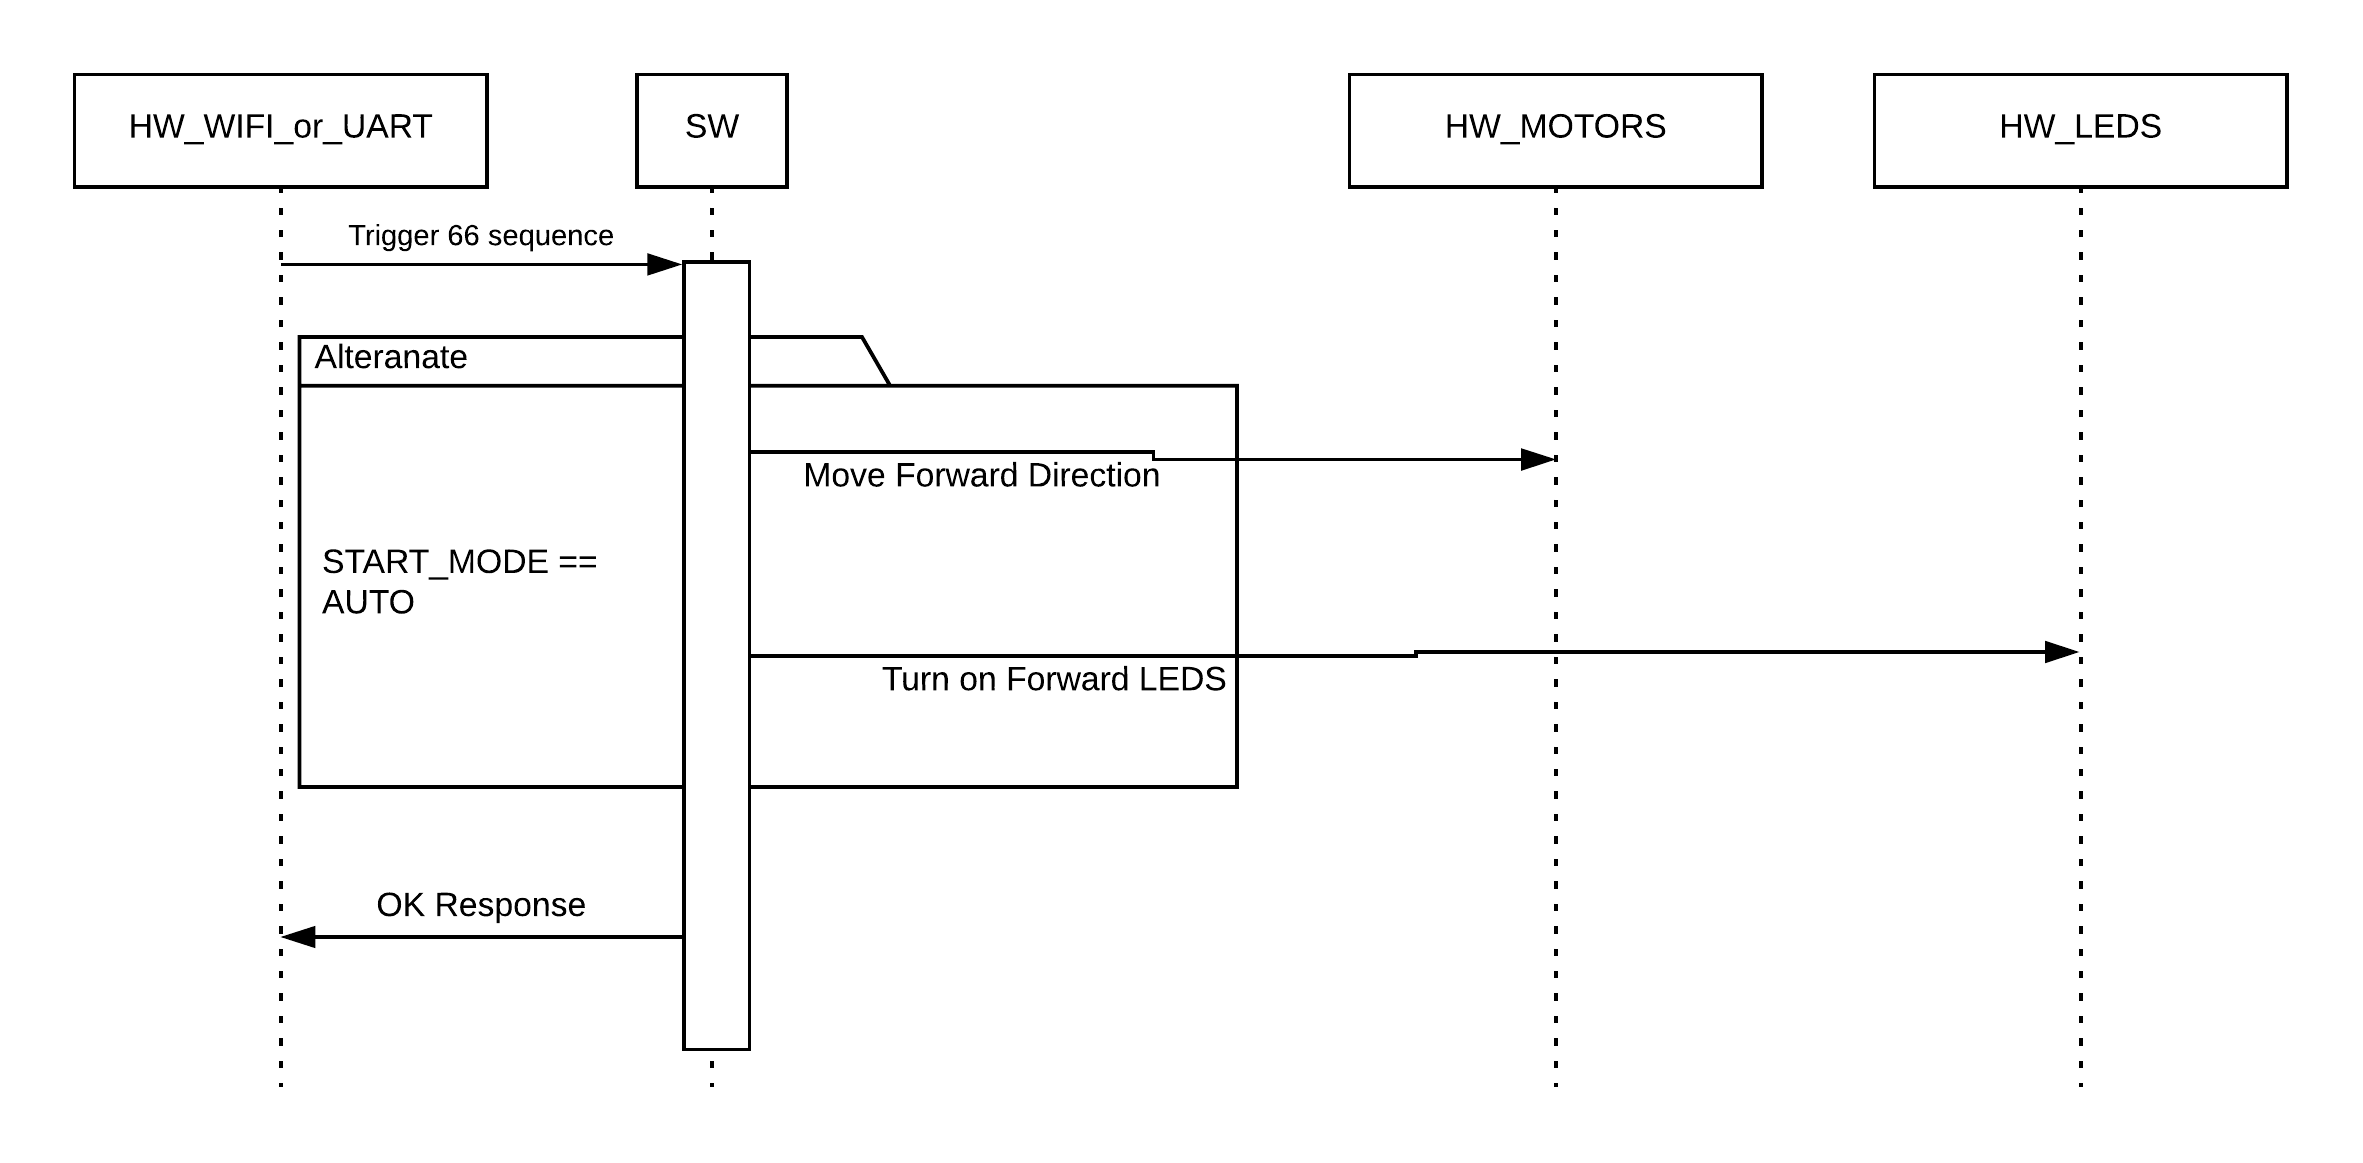
\includegraphics[width=1\columnwidth]{sequence_diagram_66.png}
\end{center}
\caption{Start 66 Signal Sequence Diagram}
\vskip\baselineskip % Leave a vertical skip below the figure
\label{fig:66_sequence}
\end{figure}

\break
\newpage

\subsection{Both Mode Diagrams}
\begin{figure}[htbp]
\begin{center}
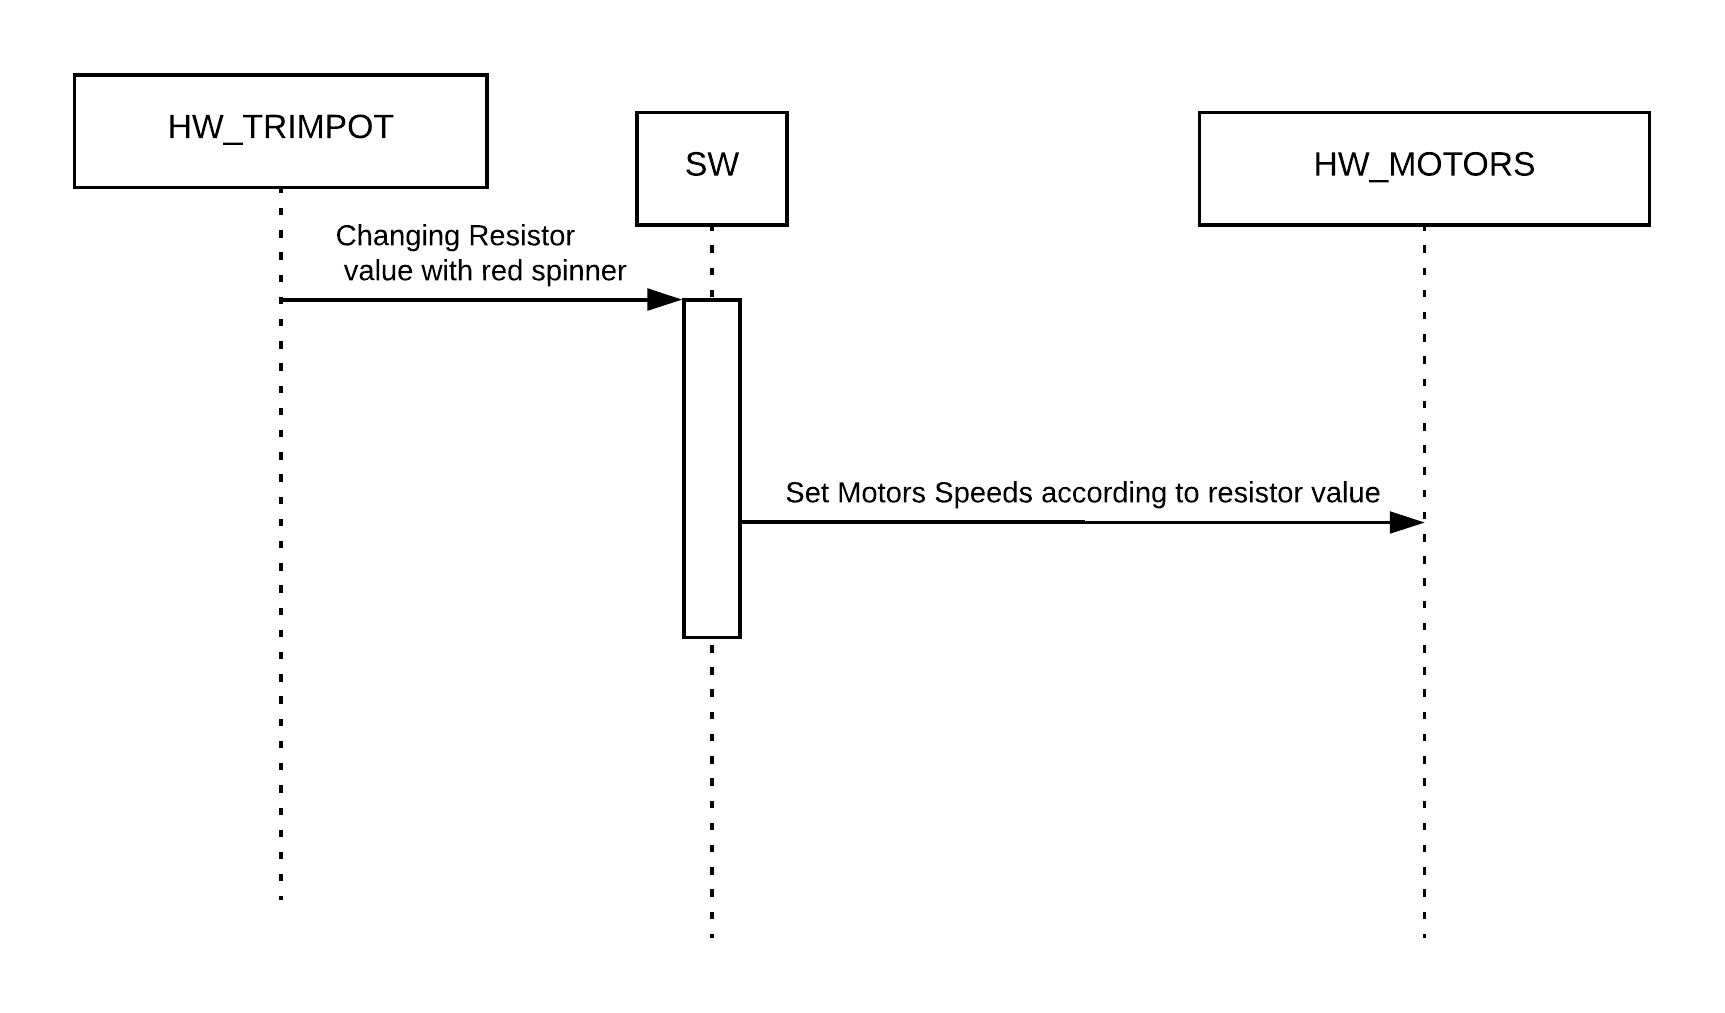
\includegraphics[width=1\columnwidth]{sequence_diagram_trimpot.png}
\end{center}
\caption{Trimpot Sequence Diagram}
\vskip\baselineskip % Leave a vertical skip below the figure
\label{fig:trimpot_sequence}
\end{figure}

\begin{figure}[htbp]
\begin{center}
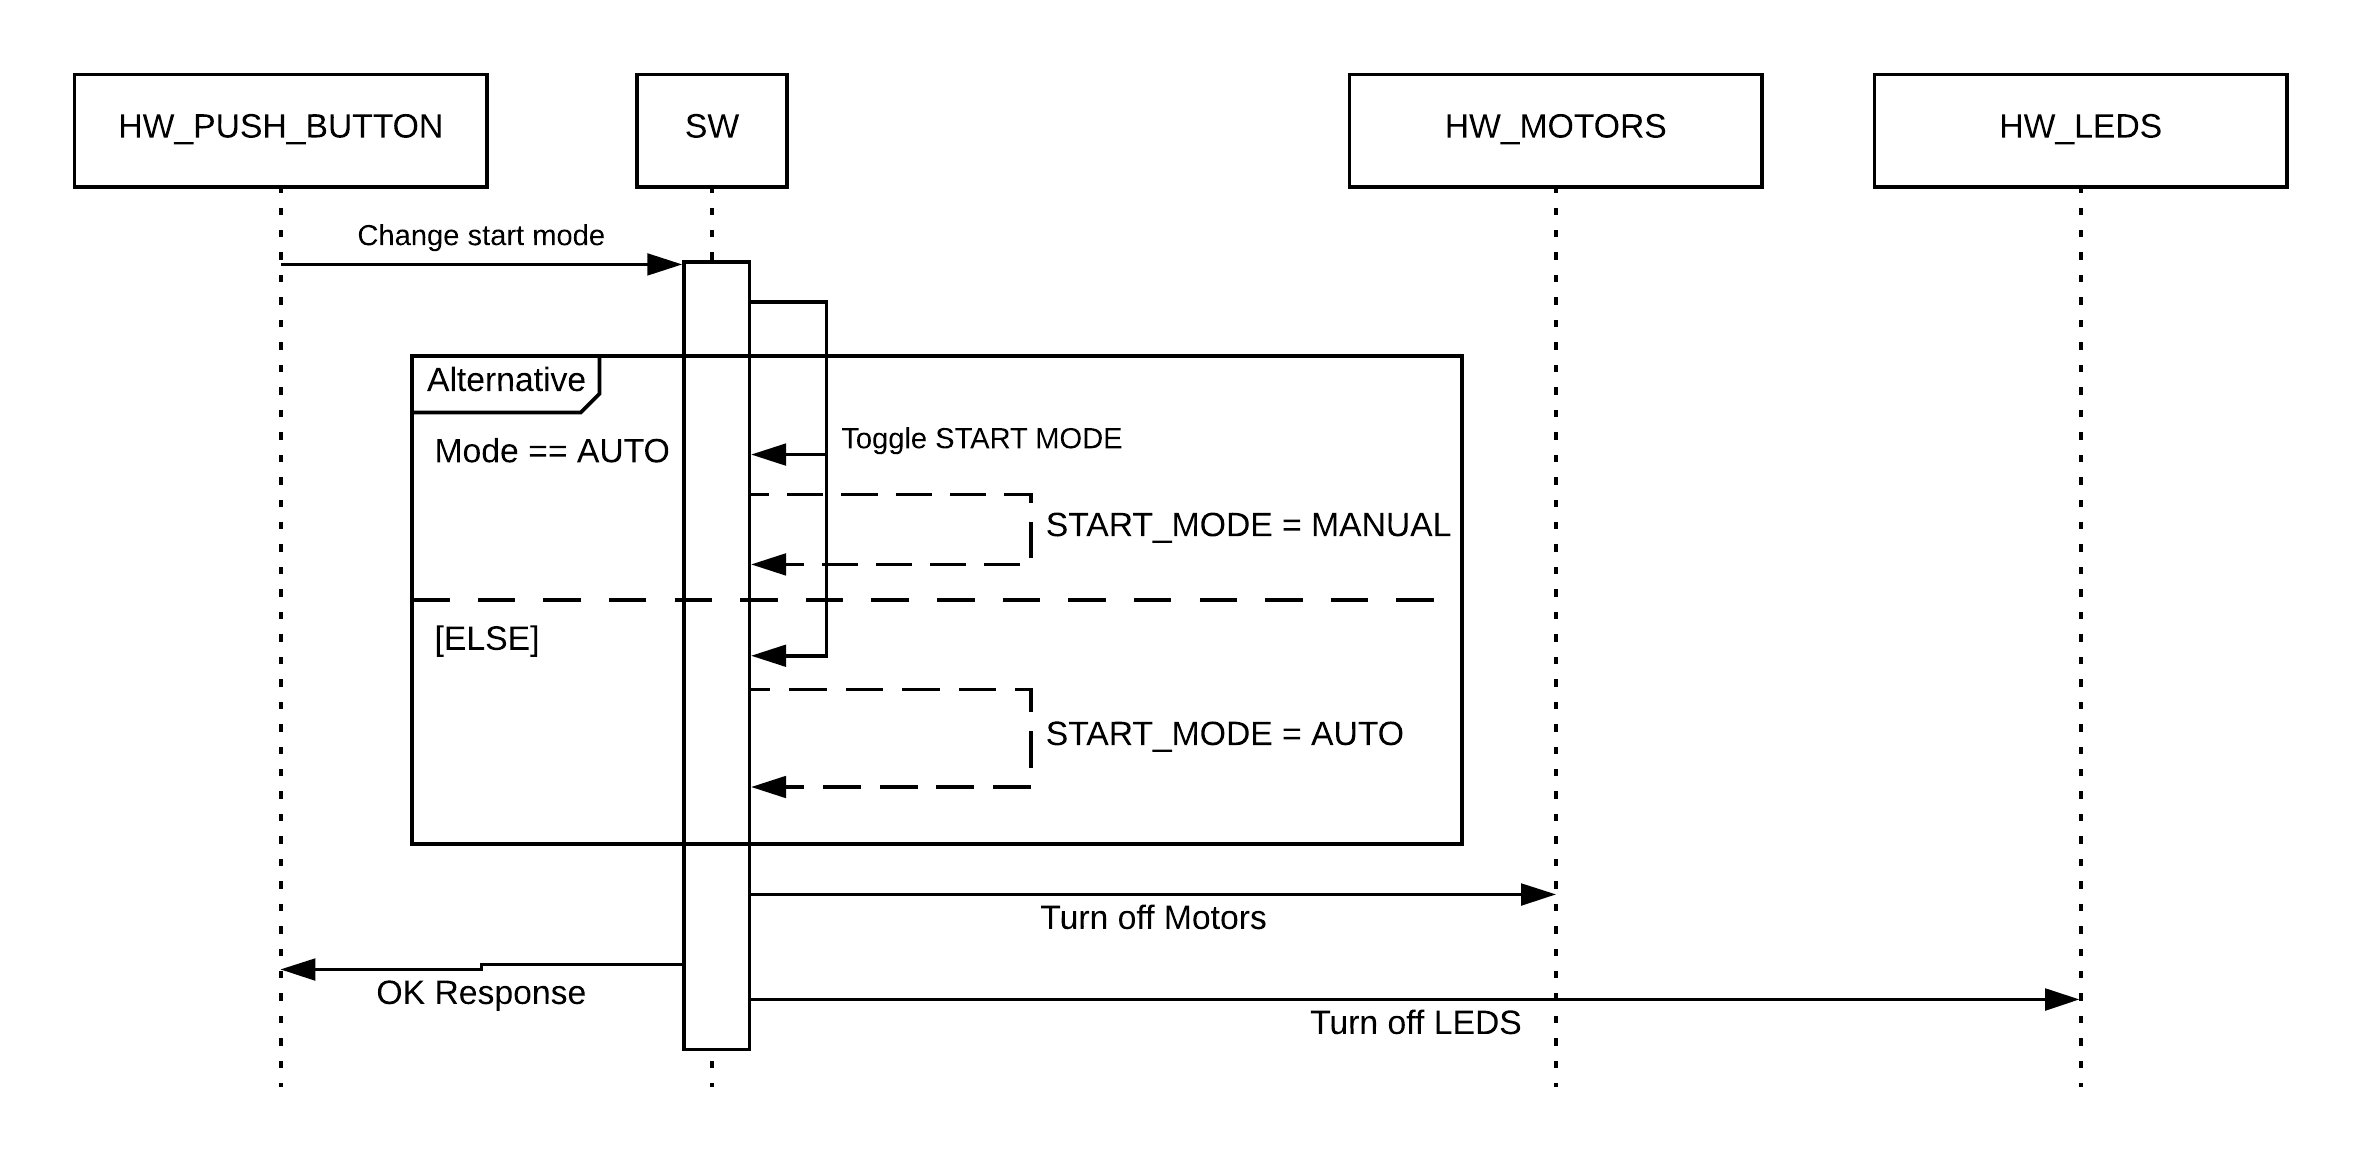
\includegraphics[width=1\columnwidth]{sequence_diagram_pushbutton.png}
\end{center}
\caption{Push Button Sequence Diagram}
\vskip\baselineskip % Leave a vertical skip below the figure
\label{fig:pushbutton_sequence}
\end{figure}

\begin{figure}[htbp]
\begin{center}
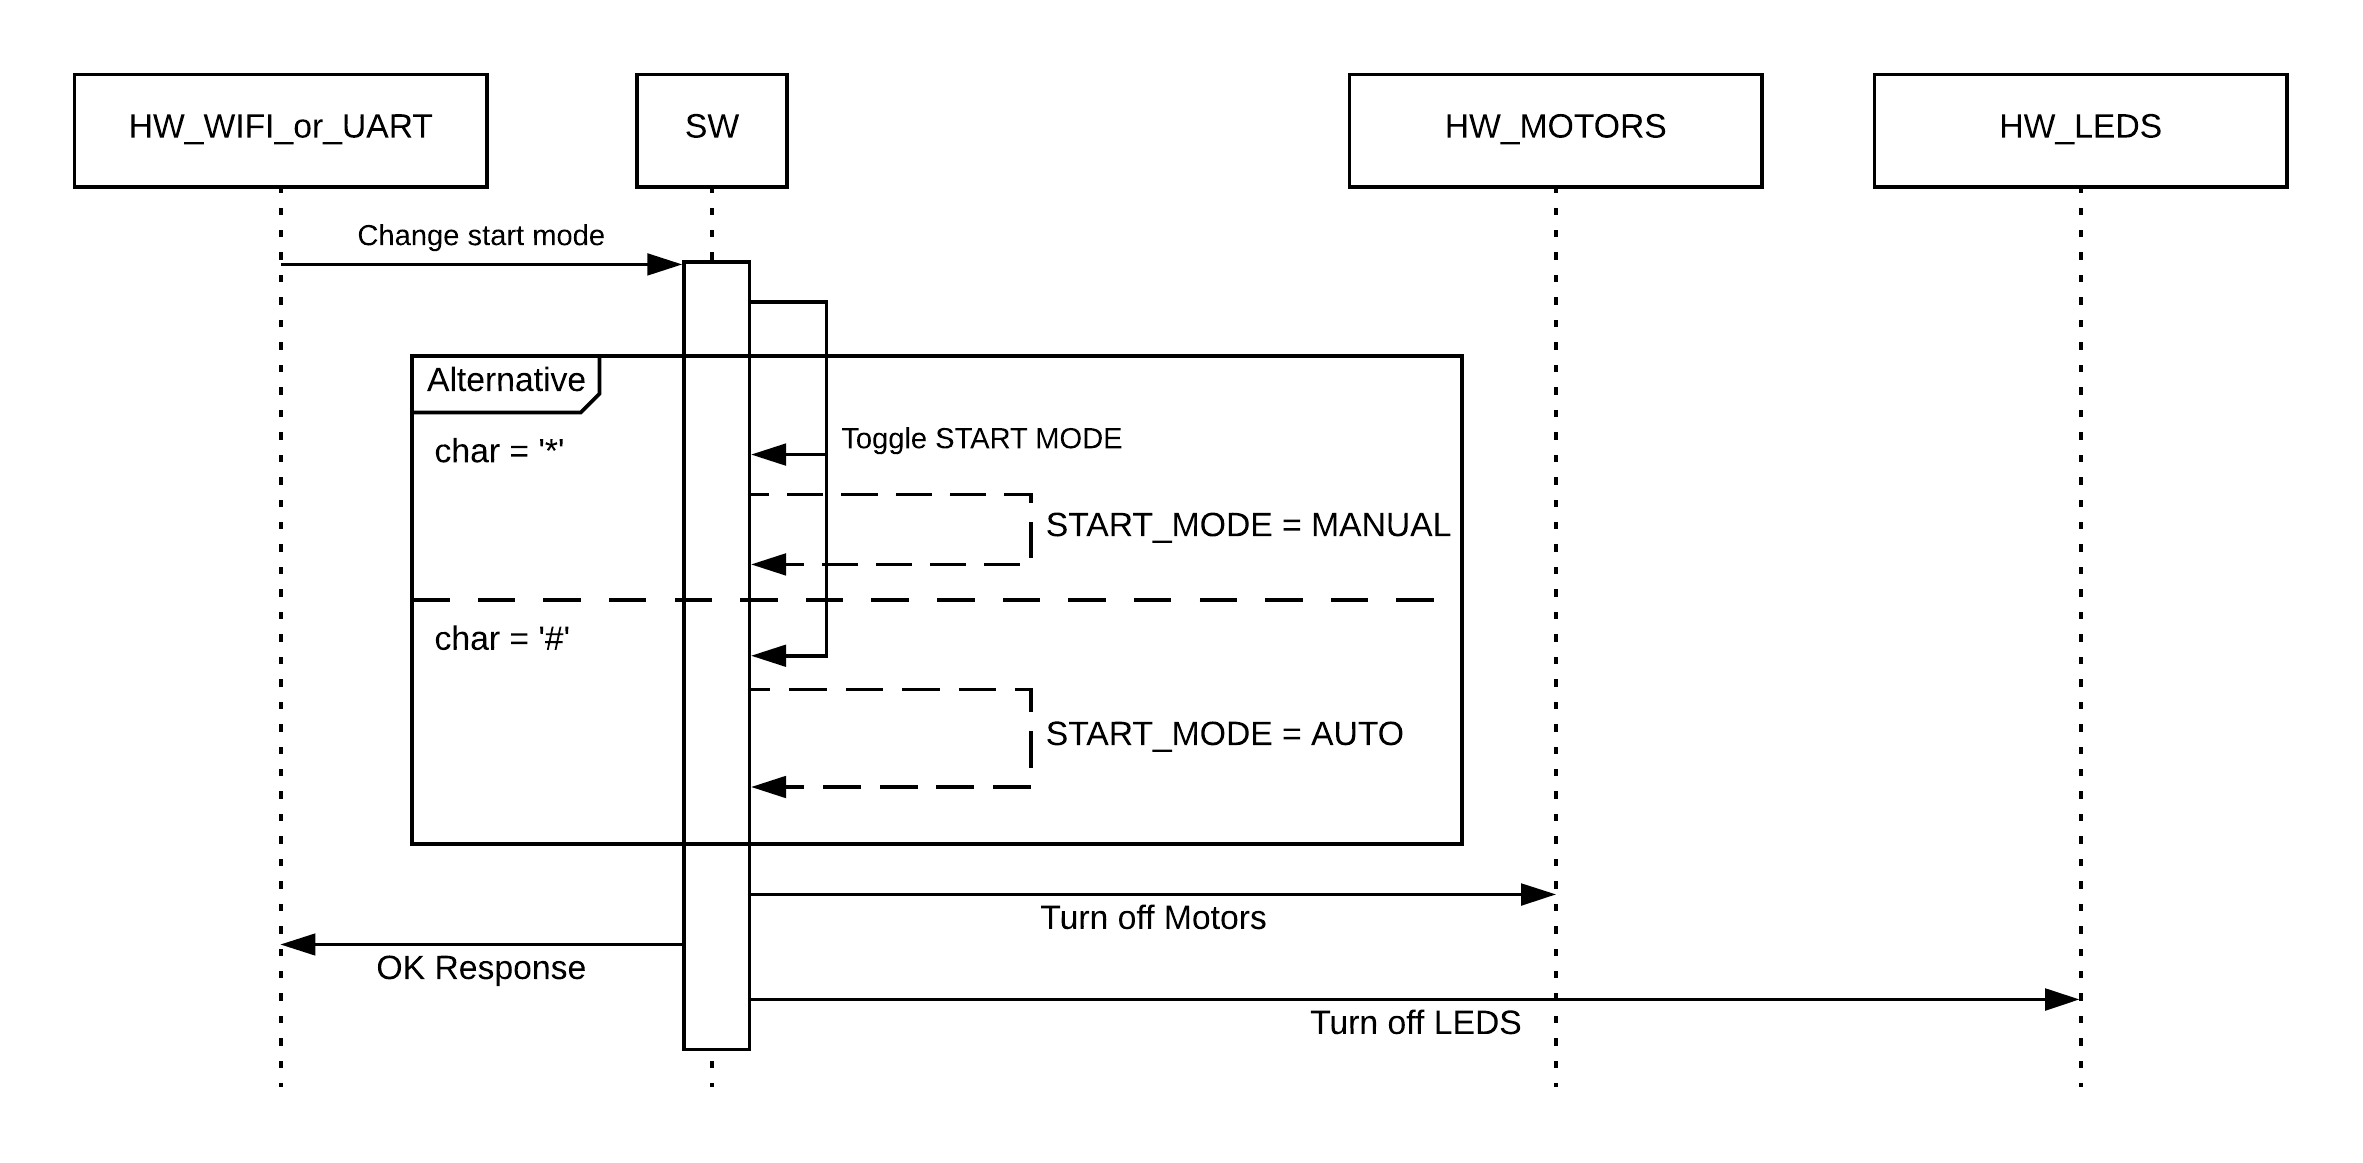
\includegraphics[width=1\columnwidth]{sequence_diagram_wifi_uart.png}
\end{center}
\caption{WIFI or UART Sequence Diagram}
\vskip\baselineskip % Leave a vertical skip below the figure
\label{fig:wifi_or_uart_sequence}
\end{figure}

\newpage
\newpage
\section{LED Connections}

\begin {table}[H]
\begin {center}
\begin{tabular}{|p{3cm}|p{3cm}|p{4cm}|p{3cm}|} 
\hline 
\textbf{LED Name} & \textbf{LPC4088 Pin} & \textbf{Pin Functionality} & \textbf{Reason} \\ 
\hline 
Forward Left & P1.5 & GPIO & Close 4 Pins \\ 
\hline 
Forward Right & P1.6 & GPIO & Close 4 Pins  \\ 
\hline 
Backward Right & P1.7 & GPIO & Close 4 Pins  \\ 
\hline 
Backward Left & P1.11 & GPIO & Close 4 Pins  \\ 
\hline 
\end{tabular}
\end {center}
\caption {LED Connections}
\end {table}

\begin{figure}[htbp]
\begin{center}
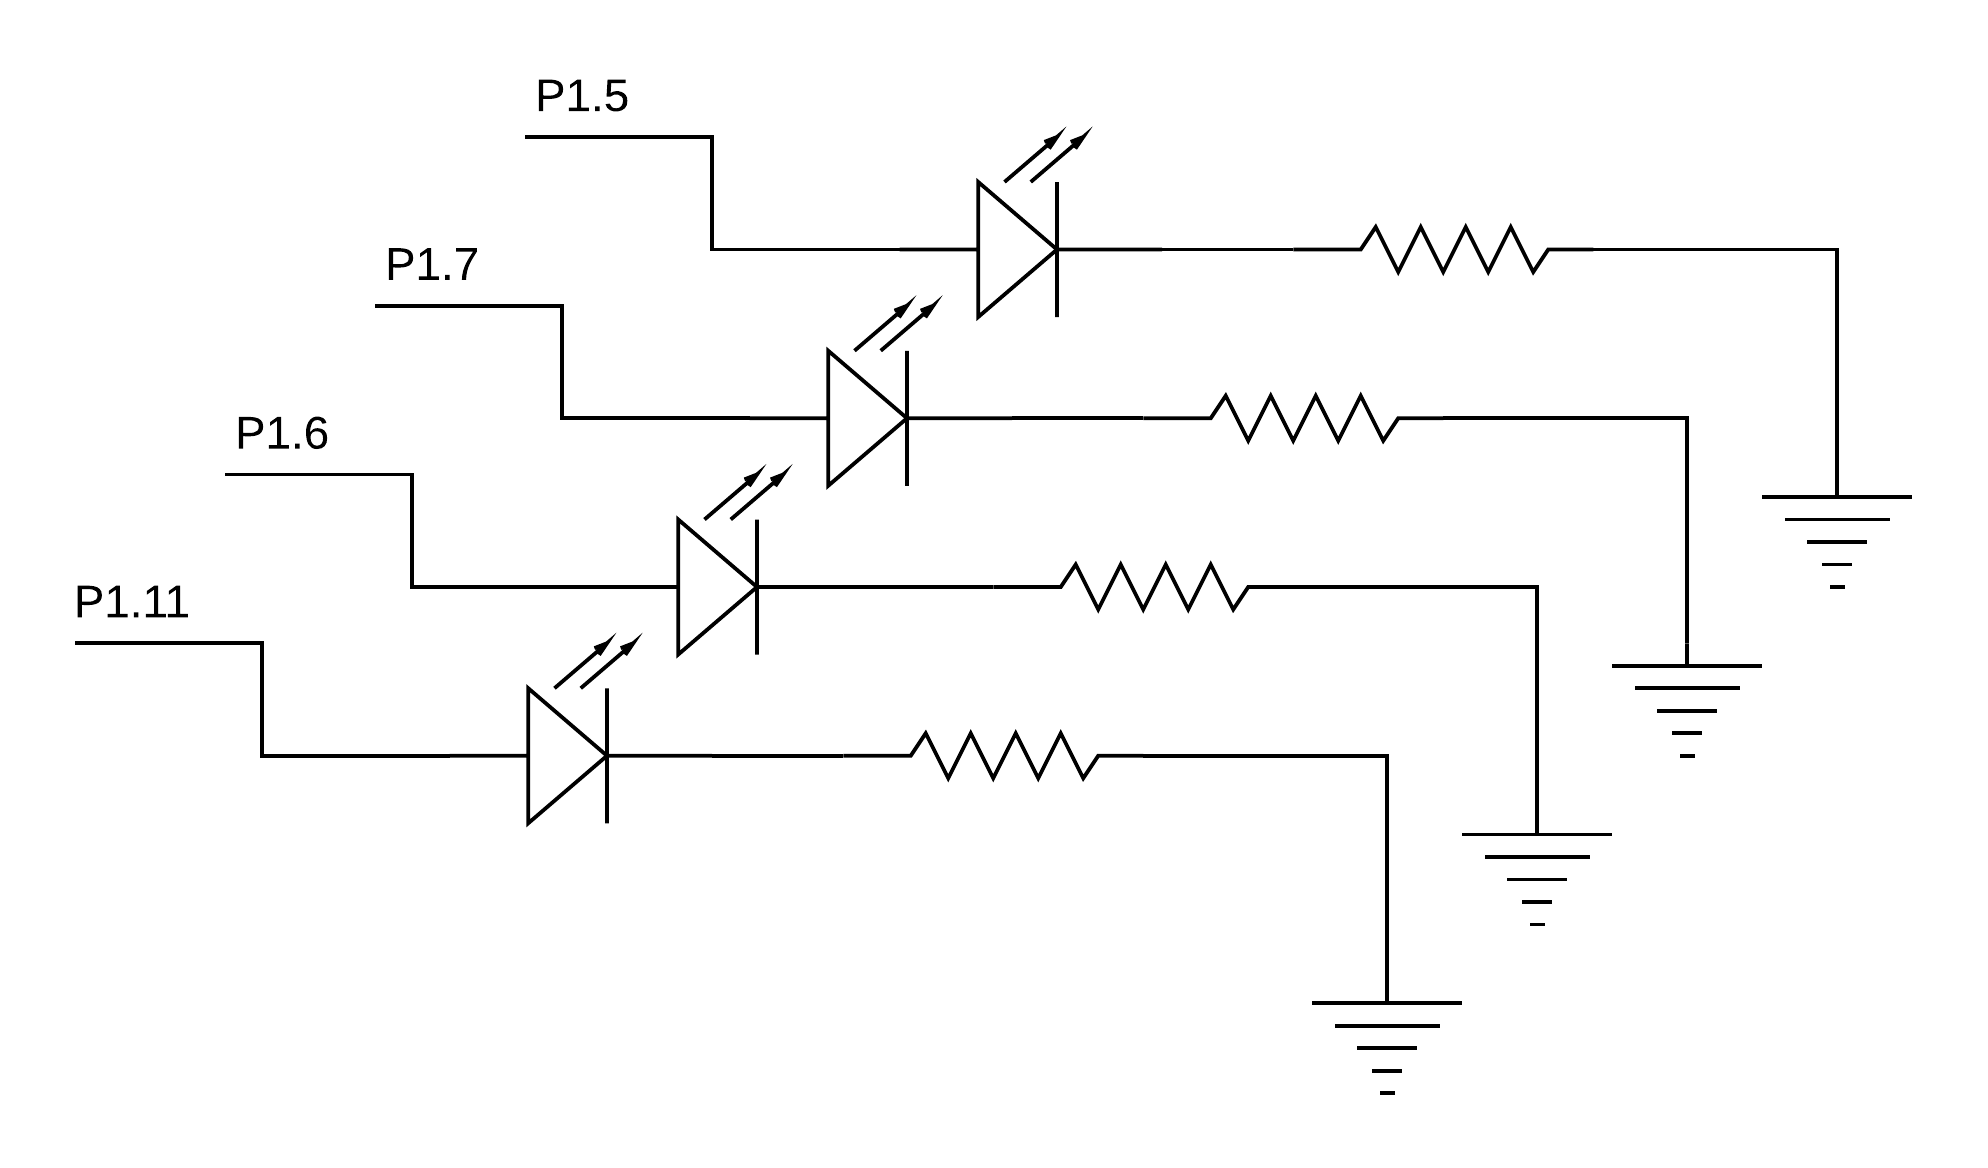
\includegraphics[width=1\columnwidth]{led_circuits.png}
\end{center}
\caption{LED Circuits}
\vskip\baselineskip % Leave a vertical skip below the figure
\label{fig:led_circuits}
\end{figure}

\newpage
\newpage
\section{Motor - Speed Sensor Connection}

\begin {table}[H]
\begin {center}
\begin{tabular}{|p{5cm}|p{3cm}|p{4cm}|p{3cm}|} 
\hline 
\textbf{Speed Sensor Name} & \textbf{LPC4088 Pin} & \textbf{Pin Functionality} & \textbf{Reason} \\ 
\hline 
Speed Sensor Left & P0.4 & T2\_CAP0 & Availability of only input for Timer 2, channel 0. \\ 
\hline 
Speed Sensor Rigth & P0.5 & T2\_CAP1 & Availability of only input for Timer 2, channel 1.  \\ 
\hline 
\end{tabular}
\end {center}
\caption {Sensor Table}                 
\end {table}

\newpage
\newpage
\section{Motor - Driver Connection}

\begin {table}[H]
\begin {center}
\begin{tabular}{|p{7cm}|p{6cm}|} 
\hline 
\textbf{Motor Terminal} & \textbf{Motor Driver Terminal} \\ 
\hline 
 Motor A Red (Left Motors +) & Output A+(OUT1) \\ 
\hline 
 Motor A Black (Left Motors -) & Output A-(OUT2)  \\ 
\hline 
 Motor B Red (Right Motors +) & Output B+(OUT3) \\ 
 \hline 
 Motor B Black (Right Motors -) & Output B-(OUT4) \\ 
\hline 
\end{tabular}
\end {center}
\caption {Motor - Driver Table}
\end {table}

\newpage
\newpage
\section{Driver - Board Connection}

\begin {table}[H]
\begin {center}
\begin{tabular}{|p{3cm}|p{3cm}|p{4cm}|p{3cm}|} 
\hline 
\textbf{Motor Driver Pin Name} & \textbf{LPC4088 Pin} & \textbf{Pin Functionality} & \textbf{Reason} \\ 
\hline 
EnA & P1.2 & PWM0\_1 & Adjacent 2 PWM0 Pins \\ 
\hline 
In1 & P0.9 & GPIO & Adjacent 4 GPIO Pins  \\ 
\hline 
In2 & P0.8 & GPIO & Adjacent 4 GPIO Pins  \\ 
\hline 
EnB & P1.3 & PWM0\_2 & Adjacent 2 PWM0 Pins  \\ 
\hline 
In3 & P0.1 & GPIO & Adjacent 4 GPIO Pins  \\ 
\hline 
In4 & P0.0 & GPIO & Adjacent 4 GPIO Pins  \\ 
\hline
\end{tabular}
\end {center}
\caption {Motor Driver Connections}
\end {table}

\newpage
\newpage

\section{Ultrasonic Sensor - Board Connection}

\begin {table}[H]
\begin {center}
\begin{tabular}{|p{5cm}|p{4cm}|p{4cm}|} 
\hline 
\textbf{Ultrasonic Sensor Pin Name} & \textbf{LPC4088 Pin} & \textbf{Pin Functionality} \\ 
\hline 
Trigger & P0.7 & T2\_MAT1 \\ 
\hline 
Echo & P0.24 & T3\_CAP1 \\ 
\hline
\end{tabular}
\end {center}
\caption {Ultrasonic Sensor Connections}
\end {table}

\begin{figure}[htbp]
\begin{center}
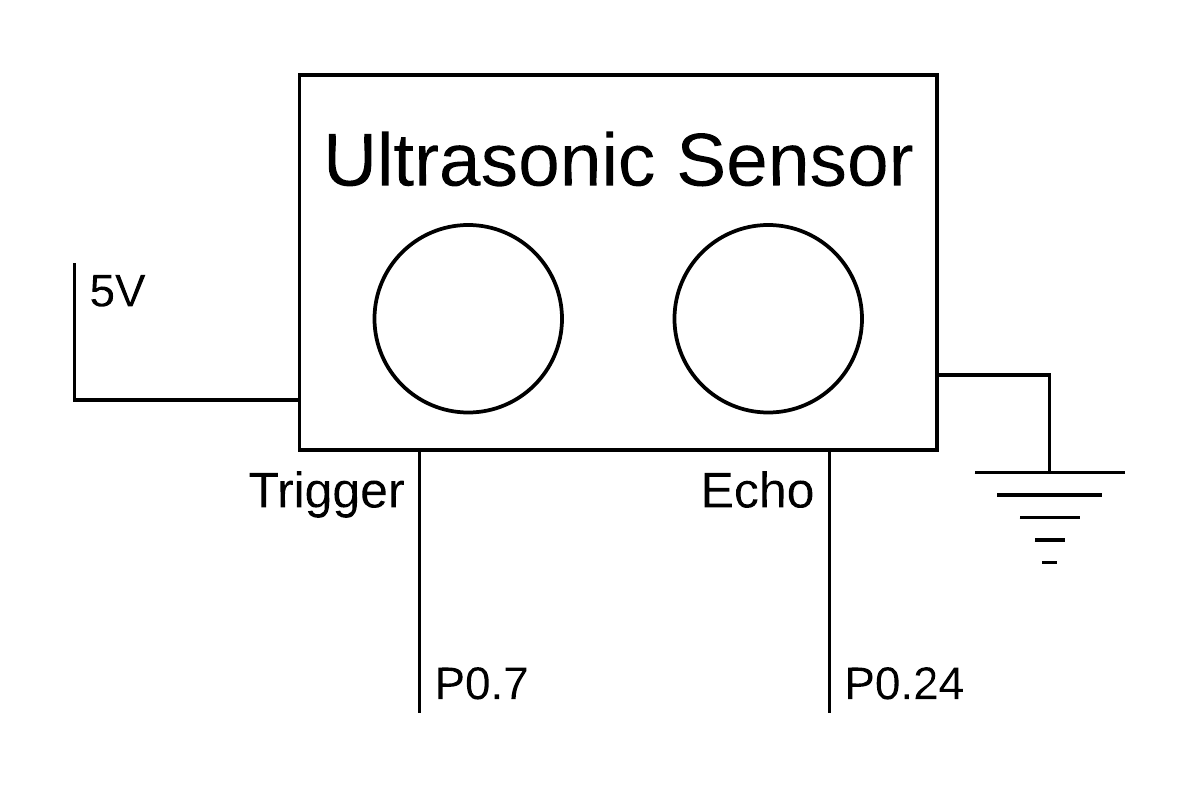
\includegraphics[width=1\columnwidth]{ultrasonic.png}
\end{center}
\caption{Ultrasonic Sensor Circuits}
\vskip\baselineskip % Leave a vertical skip below the figure
\label{fig:ultrasonic_circuits}
\end{figure}

\newpage
\newpage

\section{LDR Resistors - Board Connection}

\begin {table}[H]
\begin {center}
\begin{tabular}{|p{5cm}|p{4cm}|p{4cm}|} 
\hline 
\textbf{LPC4088 Pin} & \textbf{Pin Functionality} & \textbf{Name} \\ 
\hline 
P0.25 & ADC Channel 2 & Left LDR \\ 
\hline 
P0.26 & ADC Channel 3 & Right LDR \\ 
\hline
\end{tabular}
\end {center}
\caption {LDR Resistors Connections}
\end {table}

\begin{figure}[htbp]
\begin{center}
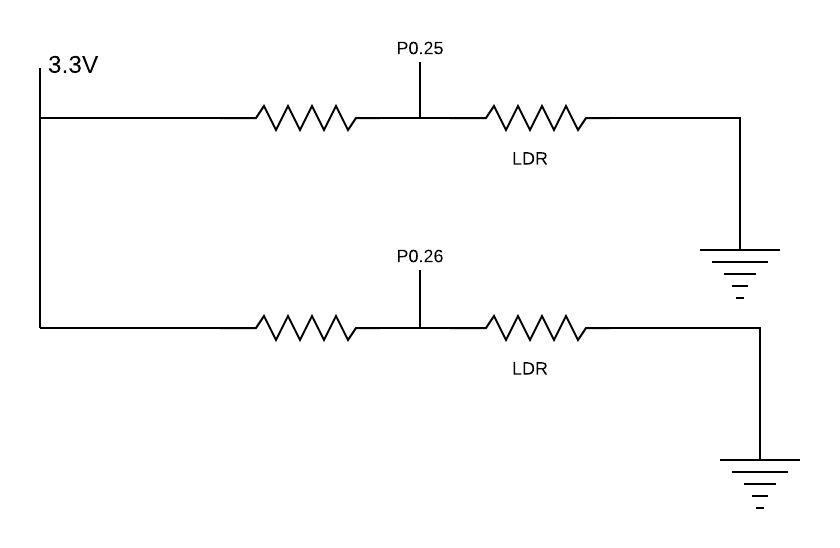
\includegraphics[width=1\columnwidth]{ldr.png}
\end{center}
\caption{LDR Circuits}
\vskip\baselineskip % Leave a vertical skip below the figure
\label{fig:ldr_circuits}
\end{figure}

\newpage
\newpage

\section{Push Button \& Trimpot Resistors - Board Connection}

\begin {table}[H]
\begin {center}
\begin{tabular}{|p{5cm}|p{4cm}|p{4cm}|} 
\hline 
\textbf{LPC4088 Pin} & \textbf{Pin Functionality} & \textbf{Name} \\ 
\hline 
P2.10 & EINT\_0 & Push Button \\ 
\hline 
P0.22 & ADC Channel 0 & Trimpot \\ 
\hline
\end{tabular}
\end {center}
\caption {Push button and Trimpot Connections}
\end {table}

\newpage
\newpage

\section{WIFI/ UART - Board Connection}

\begin {table}[H]
\begin {center}
\begin{tabular}{|p{5cm}|p{4cm}|p{4cm}|} 
\hline 
\textbf{WIFI or UART Pin Name} & \textbf{LPC4088 Pin} & \textbf{Pin Functionality} \\ 
\hline 
TX & P0.3 & U0\_RX for UART, U3\_RX for WIFI \\ 
\hline 
RX & P0.2 & U0\_TX for UART, U3\_TX for WIFI  \\ 
\hline
\end{tabular}
\end {center}
\caption {WIFI/ UART Connections}
\end {table}

\begin{figure}[htbp]
\begin{center}
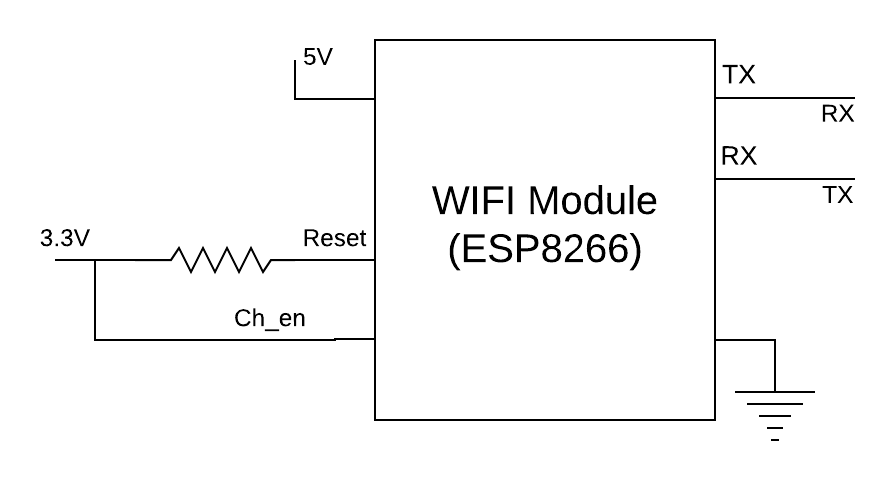
\includegraphics[width=1\columnwidth]{wifi.png}
\end{center}
\caption{WIFI Circuits}
\vskip\baselineskip % Leave a vertical skip below the figure
\label{fig:wifi_circuits}
\end{figure}

\newpage
\newpage

\section{Pin Connections - All}
\begin {table}[H]
\begin {center}
\begin{tabular}{|p{3cm}|p{3cm}|p{3cm}|p{4cm}|} 
\hline 
\textbf{LPC4088 mbed} & \textbf{LPC4088 Pin Name} & \textbf{Pin Functionality} & \textbf{Component} \\ 
\hline 
P9 & P0.0 & GPIO & Motor Driver \\ 
\hline 
P10 & P0.1 & GPIO & Motor Driver \\
\hline 
P11 & P0.9 & GPIO & Motor Driver \\ 
\hline 
P12 & P0.8 & GPIO & Motor Driver \\
\hline
P13 & P0.9 & T2\_MAT1 & Ultrasonic Sensor \\ 
\hline 
P15 & P0.8 & ADC0\_IN[0] & Trimpot \\
\hline 
P16 & P0.8 & T3\_CAP1 & Ultrasonic Sensor \\
\hline 
P17 & P0.8 & ADC0\_IN[2] & Right LDR \\
\hline 
P18 & P0.8 & ADC0\_IN[3] & Left LDR \\
\hline
P42 & P0.2 & U0\_TDX & UART Communication \\
\hline 
P41 & P0.3 & U0\_RDX & UART Communication \\
\hline
P42 & P0.2 & U3\_TDX & WIFI Communication \\
\hline 
P41 & P0.3 & U3\_RDX & WIFI Communication \\
\hline
P34 & P0.4 & T2\_CAP\_0 & Right Speed Sensor \\
\hline 
P33 & P0.5 & T2\_CAP\_1 & Left Speed Sensor \\
\hline 
P30 & P1.2 & PWM0\_1 & EnA \\
\hline 
P29 & P1.2 & PWM0\_2 & EnB \\
\hline 
P28 & P1.5 & GPIO & LED \\
\hline 
P27 & P1.6 & GPIO & LED \\
\hline 
P26 & P1.7 & GPIO & LED \\
\hline 
P25 & P1.11 & GPIO & LED \\
\hline
\end{tabular}
\end {center}
\caption {Motor Driver Connections}
\end {table}

\newpage
\newpage

\section{Expense List}
There is no extra component.

\section{Conclusion}
We implemented WIFI, UART and Basic(push button) communications. WIFI and UART use same pins so they do not work together. For determining speed and motor directions, we implemented a PID control mechanism. We had not enough time to optimize our hyper parameters (Kp, Ki, Kd). If we had adjusted these parameters, the robot would have work more accurately.

\newpage
\newpage

\section{Pseudocodes}


\begin{algorithm}
\caption{MAIN}\label{euclid}
\begin{algorithmic}[1]
\Procedure{MAIN}{}\Comment{}
\State $Init()$
\State $Wait$
\While {true}
\If {START\_MODE == AUTO} 
    \If {Joystick\_Up\_Pressed()}
		\State $TURN\_LEFT\_FLAG \gets 0$
		\State $TURN\_RIGHT\_FLAG \gets 0$
		\State $BACKWARD\_FLAG \gets 0$
		\State $FORWARD\_FLAG \gets 1$
		\State $MOTORDirection(0, FORWARD);$
		\State $MOTORDirection(1, FORWARD);$
		\State $LEDAdjuster(FORWARD_LED);$
	\EndIf
	\State $break;$
\EndIf
\EndWhile
\If {START\_MODE == MANUAL} 
    \State $Update()$
\EndIf
\EndProcedure
\end{algorithmic}
\end{algorithm}

\begin{algorithm}
\caption{Init}\label{euclid}
\begin{algorithmic}[1]
\Procedure{Initialize}{}\Comment{}
    \State $GPIO\_Init()$
    \State $PWM\_Init()$
    \State $External\_Init()$
    \If {WIFI\_COMM}
        \State $ESP8266\_Init()$
        \State $Connect WIFI$
    \Else
    \If{UART\_COMM}
        \State $Serial\_Init()$
    \EndIf
    \EndIf
    
    \State $TIMER0\_Init()$
    \State $TIMER1\_Init()$
    \State $TIMER2\_Init()$
    \State $TIMER3\_Init()$
    \State $ADC\_Init()$
\EndProcedure
\end{algorithmic}
\end{algorithm}

\begin{algorithm}
\caption{UPDATE}\label{euclid}
\begin{algorithmic}[1]
\Procedure{UPDATE}{}\Comment{}
    \If {Joystick-Center-Pressed}
        \State $Motor\_Direction(1,STOP)$
        \State $Motor\_Direction(0,STOP)$
        \State $PWM\_MOTOR\_Write(0,0)$
        \State $PWM\_MOTOR\_Write(0,1)$
        \State $Led\_Adjuster(STOP\_LED)$ 
    \EndIf
    \If {Joystick-Up-Pressed}
        \State $Motor\_Direction(1,FORWARD)$
        \State $Motor\_Direction(0,FORWARD)$
        \State $PWM\_MOTOR\_Write(0,0)$
        \State $PWM\_MOTOR\_Write(0,1)$
        \State $Led\_Adjuster(FORWARD\_LED)$ 
    \EndIf
    \If {Joystick-Down-Pressed}
        \State $Motor\_Direction(1,BACKWARD)$
        \State $Motor\_Direction(0,BACKWARD)$
        \State $Led\_Adjuster(BACKWARD\_LED)$ 
    \EndIf
    \If {Joystick-Right-Pressed}
        \State $Motor\_Direction(1,BACKWARD)$
        \State $Motor\_Direction(0,FORWARD)$
        \State $LedAdjuster(RIGHT\_BLINKER)$ 
    \EndIf
    \If {Joystick-Left-Pressed}
        \State $Motor\_Direction(1,FORWARD)$
        \State $Motor\_Direction(0,BACKWARD)$
        \State $PWM\_MOTOR\_Write(0,0)$
        \State $PWM\_MOTOR\_Write(0,1)$
        \State $Led\_Adjuster(LEFT\_BLINKER)$ 
    \EndIf
\EndProcedure
\end{algorithmic}
\end{algorithm}

\begin{algorithm}
\caption{Set Speed}\label{euclid}
\begin{algorithmic}[1]
\Procedure{setSpeed}{}\Comment{}
\If { FORWARD\_FLAG }
    \State $scale(LEFT\_LDR)$
    \State $scale(RIGHT\_LDR)$
    \State $inc = pid(ADC\_LEFT_LDR - ADC\_RIGHT\_LDR - 200)$
    \State $rightSpeed = ROBOT\_SPEED + inc$
    \State $leftSpeed  \gets ROBOT\_SPEED - inc$
    
    \If { leftSpeed > 100 }
        \State $rightSpeed \gets rightSpeed * 100 / leftSpeed$
        \State $leftSpeed \gets 100$
        \If{rightSpeed < -100}
            \State $leftSpeed \gets leftSpeed * 100 / -rightSpeed$
            \State $rightSpeed \gets -100$
        \EndIf
    \EndIf
    
     \If { rightSpeed > 100 }
        \State $leftSpeed \gets leftSpeed * 100 / rightSpeed$
        \State $rightSpeed \gets 100$
        \If {leftSpeed < -100}
            \State $rightSpeed \gets rightSpeed * 100 / -leftSpeed$
            \State $leftSpeed \gets -100$
        \EndIf
    \EndIf
    
    \State $\textit{setMotor(1, rightSpeed)}$
    \State $\textit{setMotor(1, leftSpeed)}$
\Else
    \State $\textit{PWM\_MOTOR\_Write(ROBOT\_SPEED, 0)}$
    \State $\textit{PWM\_MOTOR\_Write(ROBOT\_SPEED, 1)}$
\EndIf

\EndProcedure
\end{algorithmic}
\end{algorithm}

\begin{algorithm}
\caption{ADC\_IRQHandler}\label{euclid}
\begin{algorithmic}[1]
\Procedure{Interrupt}{}\Comment{}
\If {ADC-DR0}
    \State $TRIMPOT \gets ADC-DR[0]>>4$
\EndIf
\If {ADC-DR2}
    \State $\textit{RIGHT\_LDR} \gets ADC-DR[2]>>4$
\EndIf
\If {ADC-DR3}
    \State $\textit{LEFT\_LDR} \gets ADC-DR[3]>>4$
\EndIf
\EndProcedure
\end{algorithmic}
\end{algorithm}

\begin{algorithm}
\caption{Set Motor}\label{euclid}
\begin{algorithmic}[1]
\Procedure{setMotor}{$MOTOR\_TYPE, speed$}\Comment{}
\If {speed < 0}
    \State $\textit{MOTOR\_Direction(MOTOR\_TYPE, BACKWARD)}$
    \State $speed \gets -speed$
\Else
    \State $\textit{MOTOR\_Direction(MOTOR TYPE, FORWARD)}$
\EndIf
\If {speed > 100}
    \State $speed \gets 100$
\EndIf
\State $\textit{PWM\_MOTOR\_Write(speed, MOTOR TYPE)}$
    
\EndProcedure
\end{algorithmic}
\end{algorithm}

\begin{algorithm}
\caption{PWM\_MOTOR\_WRITE}\label{euclid}
\begin{algorithmic}[1]
\Procedure{MOTOR}{}\Comment{}
\If{T\_ON > 100}
    \State $T\_ON \gets 100$
\EndIf
\If{T\_ON == PWM0-MR0}
    \State $T-ON++$
\EndIf
\If{MOTOR\_TYPE == 0}
    \State $PWM0-MR1 \gets T\_ON $
\EndIf
\If{MOTOR\_TYPE == 0}
    \State $PWM0-MR2 \gets T\_ON $
\EndIf
\State $PWM0-LER \gets MOTOR\_TYPE + 1 $
\EndProcedure
\end{algorithmic}
\end{algorithm}

\begin{algorithm}
\caption{TIMER0\_IRQHandler}\label{euclid}
\begin{algorithmic}[1]
\Procedure{Interrupt}{}\Comment{}
 \If {COMM\_TYPE == WIFI\_COMM and count == 300}
    \State $\textit{Call procedure WIFI check}$
\EndIf
\State $ADC\_START$
\EndProcedure
\end{algorithmic}
\end{algorithm}

\begin{algorithm}
\caption{TIMER1\_IRQHandler}\label{euclid}
\begin{algorithmic}[1]
\Procedure{Interrupt}{}\Comment{}

 \If {TURN\_LEFT\_FLAG != 0}
\State $\textit{TURN\_LEFT\_FLAG} ++$
\State $\textit{LED\_Change (TURN\_RIGHT\_FLAG)}$
\EndIf
\State Clear the interrupt flag for MAT channel 0 event

\EndProcedure
\end{algorithmic}
\end{algorithm}


\begin{algorithm}
\caption{TIMER2\_IRQHandler}\label{euclid}
\begin{algorithmic}[1]
\Procedure{Interrupt}{}\Comment{}

\If {TIMER2-IR  1}
    \If {TIMER2-MR1 == 10 }
        \State $\textit{Change MR1 Register Value for 60000}$
        \State $ultrasonicSensorEdgeCount \gets 0$
    \Else \State $\textit{Change MR1 Register Value for 10}$
    \EndIf
    
     \State $\textit{Reset Timer Counter and Prescale Counter for Timer2}$
     \State $\textit{Start timer again}$
     \State $\textit{Remove reset on Timer2}$
      \State $\textit{Clear IR Register Flag for Corresponding Interrupt}$
     \State Clear the interrupt flag for MAT channel 0 event
\EndIf
\EndProcedure
\end{algorithmic}
\end{algorithm}

\begin{algorithm}
\caption{TIMER3\_IRQHandler}\label{euclid}
\begin{algorithmic}[1]
\Procedure{Interrupt}{}\Comment{}

\If {ultrasonicSensorEdgeCount == 0}
     \State $\textit{Store the rising time into ultrasonicSensorRisingTime variable}$
\EndIf
\If {ultrasonicSensorEdgeCount == 1}
    \If {ultrasonicSensorDistance < OBSTACLE\_DISTANCE}
        \State $LED\_Adjuster(Backward\_LED)$
        \State $MOTOR\_Direction(Backward)$
        \State $Go Back$
    \EndIf
    \If {ultrasonicSensorDistance > OBSTACLE\_DISTANCE}
        \State $LEDAdjuster Forward LED$
        \State $MOTORDirection Forward$
        \State $Go Back$
    \EndIf
\EndIf
\State $ultrasonicSensorEdgeCount++$

\EndProcedure
\end{algorithmic}
\end{algorithm}

\begin{algorithm}
\caption{ESP8266}\label{euclid}
\begin{algorithmic}[1]
\Procedure{sendCommand}{$command$}\Comment{}
\For{index < ESP8266BufferSize}
    \State $esp8266Response[index] \gets 0$
\EndFor
\State $esp8266ResponseStartIndex \gets esp8266CurrentBufferIndex$
\State $ESP8266\_Write(command)$
\EndProcedure
\Procedure{waitResponseEnd}{$command$}\Comment{}
\For{;;}
    \For{esp8266ResponseCurrentIndex < responseEndIndex}
    \State $bufferIndex = StartIndex + CurrentIndex$
    \State $esp8266Response[CurrentIndex] = Buffer[bufferIndex]$
    \EndFor
\EndFor
\EndProcedure
\Procedure{readResponse}{}\ Comment{}
\State $esp8266CurrentBufferIndex \gets 0$
\For {index < ESP8266BufferSize}
    \State $esp8266Buffer[index] \gets 0$
\EndFor
\While {ESP8266\_UART-LSR}
    \If {data != 'n'}
        \State $esp8266Buffer[esp8266CurrentBufferIndex] = data $
        \State $esp8266CurrentBufferIndex++$
    \EndIf
\EndWhile
\EndProcedure

\Procedure{readData}{}\Comment{}
\If {data != 'n'}
        \State $esp8266Buffer[esp8266CurrentBufferIndex] = data $
        \State $esp8266CurrentBufferIndex++$
\EndIf
\EndProcedure
\end{algorithmic}
\end{algorithm}


\begin{algorithm}
\caption{PID}\label{euclid}
\begin{algorithmic}[1]
\Procedure{pid}{$error$}\Comment{}

\State $combinedPIDValues \gets 0$
\State $combinedPIDValues \gets Kp * error$
\State $total\_error \gets total\_error * 3 / 4 + error * 10$
\State $combinedPIDValues \gets combinedPIDValues + total\_error* Ki$
\State $combinedPIDValues \gets combinedPIDValues + (Kd * (error - prev_error)) / 10$
\State $prev\_error \gets error$

\EndProcedure
\end{algorithmic}
\end{algorithm}

\begin{algorithm}
\caption{WIFI CHECK}\label{euclid}
\begin{algorithmic}[1]
\Procedure{WIFI CHECK}{}\Comment{}
    \State $\textit{Start TCP Connection}$
    \State $\textit{Get Information from WIFI}$
    \State $\textit{Change to ROBOT-MODE or start robot}$
\EndProcedure
\end{algorithmic}
\end{algorithm}

\begin{algorithm}
\caption{Change Start Mode}\label{euclid}
\begin{algorithmic}[1]
\Procedure{Change Start Mode}{$state$}\Comment{}
    \State $StartMode \gets state$
    \State $Stop Motors and LEDs$
    
    \If {COMM\_TYPE == WIFI\_COMM}
        \State $\textit{Send Information about state via wifi}$
    \EndIf
\EndProcedure
\end{algorithmic}
\end{algorithm}

\end{document}
%
% End of fbeman.tex
